\makeatletter
\@ifundefined{standalonetrue}{\newif\ifstandalone}{}
\@ifundefined{section}{\standalonetrue}{\standalonefalse}
\makeatother
\ifstandalone
\documentclass{report}

\usepackage{textcase}
%\usepackage{hyperref}
%\hypersetup{breaklinks=true}


% Added packages
\usepackage[usenames]{color}
\usepackage{amsfonts, amsmath, amssymb, graphics}

% NOTE: bibentry MUST appear before the hyperref or build will fail
\usepackage{bibentry}
\nobibliography*
\usepackage[square,sort,comma,numbers]{natbib}
  
\usepackage{float}
\usepackage[
	hidelinks,%
    %hyperindex=true,		% Make numbers of index links as well
   	backref=page, 		% Provide page listing where refs occur in the bibliography
	%breaklinks=true,
    %colorlinks,%
    %citecolor=green,%
    %filecolor=blue,%
    %linkcolor=red,%
    %urlcolor=red, 
]{hyperref}

\usepackage{dsfont}
%%%% USEPACKAGES for MACROS %%%%%
\usepackage{algpseudocode}
\usepackage[chapter]{algorithm}
%\usepackage{caption}
\usepackage{subcaption}
\usepackage{url}

\usepackage{array}
\usepackage{arydshln}
\usepackage{multirow}
\usepackage{multicol}
%\usepackage[section]{placeins}

\usepackage[usenames,dvipsnames]{color}
%\usepackage[english]{babel}
\usepackage{tabularx}
\usepackage{soul}
\usepackage{xparse}
\usepackage{listings}
%\usepackage[normalem]{ulem}



%%%%%%%%%%%%%%%
% Show a list of items "todo" or "done" 
% USAGE: 
% \begin{todolist} 
% 	\todo Something not finished
% 	\done Something finished
% \end{todolist} 
\newenvironment{todolist}{%
  \begin{list}{}{}% whatever you want the list to be
  \let\olditem\item
  \renewcommand\item{\olditem \textcolor{red}{(TODO)}: }
  \newcommand\todo{\olditem \textcolor{red}{(TODO)}: }
   \newcommand\done{\olditem \textcolor{ForestGreen}{(DONE)}: }
}{%
  \end{list}
} 
%%%%%%%%%%%%%%%

%%%%%%%%%%%%%%%
% Show a Author's Note
% USAGE: 
% \incomplete[Optional footnote message to further clarify note]{The text which is currently not finished}
\DeclareDocumentCommand \incomplete{ o m }
{%
\IfNoValueTF {#1}
{\textcolor{red}{Incomplete: \ul{#2}}} 
{\textcolor{red}{Incomplete: \ul{#2}}\footnote{Comment: #1}}%
}
%%%%%%%%%%%%%%%



%%%%%%%%%%%%%%%
% Show a Author's Note
% USAGE: 
% \authnote[Optional footnote message to further clarify note]{The note to your readers}
\DeclareDocumentCommand \authnote { o m }
{%
\IfNoValueTF {#1}
{\textcolor{blue}{Author's Note: \ul{#2}}} 
{\textcolor{blue}{Author's Note: \ul{#2}}\footnote{Comment: #1}}%
}
%%%%%%%%%%%%%%%



%%%%%%%%%%%%%%%
% Strike out text that doesn't belong in the paper
% USAGE: 
% \strike[Optional footnote to state why it doesn't belong]{Text to strike out}
\DeclareDocumentCommand \strike { o m }
{%
\setstcolor{Red}
\IfNoValueTF {#1}
{\textcolor{Gray}{\st{#2}}} 
{\textcolor{Gray}{\st{#2}}\footnote{Comment: #1}}%
}
%%%%%%%%%%%%%%%

\definecolor{light-gray}{gray}{0.95}

\newcommand{\cbox}[3]{
\ \\
\fcolorbox{#1}{#2}{
\parbox{\textwidth}{
#3
}
}
}

% Setup an environment similar to verbatim but which will highlight any bash commands we have
\lstnewenvironment{unixcmds}[0]
{
%\lstset{language=bash,frame=shadowbox,rulesepcolor=\color{blue}}
\lstset{ %
language=sh,		% Language
basicstyle=\ttfamily,
backgroundcolor=\color{light-gray}, 
rulecolor=\color{blue},
%frame=tb, 
columns=fullflexible,
%framexrightmargin=-.2\textwidth,
linewidth=0.8\textwidth,
breaklines=true,
%prebreak=/, 
  prebreak = \raisebox{0ex}[0ex][0ex]{\ensuremath{\hookleftarrow}},
%basicstyle=\footnotesize,       % the size of the fonts that are used for the code
%numbers=left,                   % where to put the line-numbers
%numberstyle=\footnotesize,      % the size of the fonts that are used for the line-numbers
%stepnumber=2,                   % the step between two line-numbers. If it's 1 each line 
                                % will be numbered
%numbersep=5pt,                  % how far the line-numbers are from the code
showspaces=false,               % show spaces adding particular underscores
showstringspaces=false,         % underline spaces within strings
showtabs=false,                 % show tabs within strings adding particular underscores
frame=single,	                % adds a frame around the code
tabsize=2,	                % sets default tabsize to 2 spaces
captionpos=b,                   % sets the caption-position to bottom
breakatwhitespace=false,        % sets if automatic breaks should only happen at whitespace
}
} { }

% Setup an environment similar to verbatim but which will highlight any bash commands we have
\lstnewenvironment{cppcode}[1]
{
%\lstset{language=bash,frame=shadowbox,rulesepcolor=\color{blue}}
\lstset{ %
	backgroundcolor=\color{light-gray}, 
	rulecolor=\color[rgb]{0.133,0.545,0.133},
	tabsize=4,
	language=[GNU]C++,
%	basicstyle=\ttfamily,
        basicstyle=\scriptsize,
        upquote=true,
        aboveskip={1.5\baselineskip},
        columns=fullflexible,
        %framexrightmargin=-.1\textwidth,
       %framexleftmargin=6mm,
        showstringspaces=false,
        extendedchars=true,
        breaklines=true,
        prebreak = \raisebox{0ex}[0ex][0ex]{\ensuremath{\hookleftarrow}},
        frame=single,
        showtabs=false,
        showspaces=false,
        showstringspaces=false,
        numbers=left,                   % where to put the line-numbers
	numberstyle=\footnotesize,      % the size of the fonts that are used for the line-numbers
	stepnumber=4,                   % the step between two line-numbers. If it's 1 each line 
                                % will be numbered
	firstnumber=#1,
         numbersep=5pt,                  % how far the line-numbers are from the code
        identifierstyle=\ttfamily,
        keywordstyle=\color[rgb]{0,0,1},
        commentstyle=\color[rgb]{0.133,0.545,0.133},
        stringstyle=\color[rgb]{0.627,0.126,0.941},
}
} { }

% Setup an environment similar to verbatim but which will highlight any bash commands we have
\lstnewenvironment{mcode}[1]
{
\lstset{ %
	backgroundcolor=\color{light-gray}, 
	rulecolor=\color[rgb]{0.133,0.545,0.133},
	tabsize=4,
	language=Matlab,
%	basicstyle=\ttfamily,
        basicstyle=\scriptsize,
        upquote=true,
        aboveskip={1.5\baselineskip},
        columns=fullflexible,
        %framexrightmargin=-.1\textwidth,
       %framexleftmargin=6mm,
        showstringspaces=false,
        extendedchars=true,
        breaklines=true,
        prebreak = \raisebox{0ex}[0ex][0ex]{\ensuremath{\hookleftarrow}},
        frame=single,
        showtabs=false,
        showspaces=false,
        showstringspaces=false,
        numbers=left,                   % where to put the line-numbers
	numberstyle=\footnotesize,      % the size of the fonts that are used for the line-numbers
	stepnumber=4,                   % the step between two line-numbers. If it's 1 each line 
                                % will be numbered
	firstnumber=#1,
         numbersep=5pt,                  % how far the line-numbers are from the code
        identifierstyle=\ttfamily,
        keywordstyle=\color[rgb]{0,0,1},
        commentstyle=\color[rgb]{0.133,0.545,0.133},
        stringstyle=\color[rgb]{0.627,0.126,0.941},
}
} { }

\newcommand{\inputmcode}[1]{%
\lstset{ %
	backgroundcolor=\color{light-gray},  %
	rulecolor=\color[rgb]{0.133,0.545,0.133}, %
	tabsize=4, %
	language=Matlab, %
%	basicstyle=\ttfamily,
        basicstyle=\scriptsize, %
        %        upquote=true,
        aboveskip={1.5\baselineskip}, %
        columns=fullflexible, %
        %framexrightmargin=-.1\textwidth,
       %framexleftmargin=6mm,
        showstringspaces=false, %
        extendedchars=true, %
        breaklines=true, %
        prebreak = \raisebox{0ex}[0ex][0ex]{\ensuremath{\hookleftarrow}}, %
        frame=single, %
        showtabs=false, %
        showspaces=false, %
        showstringspaces=false,%
        numbers=left,                   % where to put the line-numbers
	numberstyle=\footnotesize,      % the size of the fonts that are used for the line-numbers
	stepnumber=4,                   % the step between two line-numbers. If it's 1 each line 
                                % will be numbered
         numbersep=5pt,                  % how far the line-numbers are from the code
        identifierstyle=\ttfamily, %
        keywordstyle=\color[rgb]{0,0,1}, %
        commentstyle=\color[rgb]{0.133,0.545,0.133}, %
        stringstyle=\color[rgb]{0.627,0.126,0.941} %
}
\lstinputlisting{#1}%
}

%\lstset{ %
%	backgroundcolor=\color{light-gray}, 
%	rulecolor=\color[rgb]{0.133,0.545,0.133},
%	tabsize=4,
%	language=Matlab,
%%	basicstyle=\ttfamily,
%        basicstyle=\scriptsize,
%        upquote=true,
%        aboveskip={1.5\baselineskip},
%        columns=fullflexible,
%        %framexrightmargin=-.1\textwidth,
%       %framexleftmargin=6mm,
%        showstringspaces=false,
%        extendedchars=true,
%        breaklines=true,
%        prebreak = \raisebox{0ex}[0ex][0ex]{\ensuremath{\hookleftarrow}},
%        frame=single,
%        showtabs=false,
%        showspaces=false,
%        showstringspaces=false,
%        numbers=left,                   % where to put the line-numbers
%	numberstyle=\footnotesize,      % the size of the fonts that are used for the line-numbers
%	stepnumber=4,                   % the step between two line-numbers. If it's 1 each line 
%                                % will be numbered
%	firstnumber=#1,
%         numbersep=5pt,                  % how far the line-numbers are from the code
%        identifierstyle=\ttfamily,
%        keywordstyle=\color[rgb]{0,0,1},
%        commentstyle=\color[rgb]{0.133,0.545,0.133},
%        stringstyle=\color[rgb]{0.627,0.126,0.941},
%}


\newcommand{\Laplacian}[1]{\nabla^2 #1}

% set of all nodes received and contained on GPU
\newcommand{\setAllNodes}[0]{\mathcal{G}}
% set of stencil centers on GPU
\newcommand{\setCenters}[0]{\mathcal{Q}}
% set of stencil centers with nodes in \setDepend
\newcommand{\setBoundary}[0]{\mathcal{B}}
% set of nodes received by other GPUs
\newcommand{\setDepend}[0]{\mathcal{R}}
% set of nodes sent to other GPUs
\newcommand{\setProvide}[0]{\mathcal{O}}


\newcommand{\toprule}[0]{\hline}
\newcommand{\midrule}[0]{\hline\hline}
\newcommand{\bottomrule}[0]{\hline}

\newcolumntype{C}{>{\centering\arraybackslash}b{1in}}
\newcolumntype{L}{>{\flushleft\arraybackslash}b{1.5in}}
\newcolumntype{R}{>{\flushright\arraybackslash}b{1.5in}}
\newcolumntype{D}{>{\flushright\arraybackslash}b{2.0in}}
\newcolumntype{E}{>{\flushright\arraybackslash}b{1.0in}}

\DeclareSymbolFont{AMSb}{U}{msb}{m}{n}
\DeclareMathSymbol{\N}{\mathbin}{AMSb}{"4E}
\DeclareMathSymbol{\Z}{\mathbin}{AMSb}{"5A}
\DeclareMathSymbol{\R}{\mathbin}{AMSb}{"52}
\DeclareMathSymbol{\Q}{\mathbin}{AMSb}{"51}
\DeclareMathSymbol{\PP}{\mathbin}{AMSb}{"50}
\DeclareMathSymbol{\I}{\mathbin}{AMSb}{"49}
%\DeclareMathSymbol{\C}{\mathbin}{AMSb}{"43}

%%%%%% VECTOR NORM: %%%%%%%
\newcommand{\vectornorm}[1]{\left|\left|#1\right|\right|}
\newcommand{\vnorm}[1]{\left|\left|#1\right|\right|}
\newcommand{\by}[0]{\times}
\newcommand{\vect}[1]{\mathbf{#1}}
%\newcommand{\mat}[1]{\mathbf{#1}} 

%\renewcommand{\vec}[1]{ \textbf{#1} }
%%%%%%%%%%%%%%%%%%%%%%

%%%%%%% THM, COR, DEF %%%%%%%
%\newtheorem{theorem}{Theorem}[section]
%\newtheorem{lemma}[theorem]{Lemma}
%\newtheorem{proposition}[theorem]{Proposition}
%\newtheorem{corollary}[theorem]{Corollary}
%\newenvironment{proof}[1][Proof]{\begin{trivlist}
%\item[\hskip \labelsep {\bfseries #1}]}{\end{trivlist}}
%\newenvironment{definition}[1][Definition]{\begin{trivlist}
%\item[\hskip \labelsep {\bfseries #1}]}{\end{trivlist}}
%\newenvironment{example}[1][Example]{\begin{trivlist}
%\item[\hskip \labelsep {\bfseries #1}]}{\end{trivlist}}
%\newenvironment{remark}[1][Remark]{\begin{trivlist}
%\item[\hskip \labelsep {\bfseries #1}]}{\end{trivlist}}
%\newcommand{\qed}{\nobreak \ifvmode \relax \else
%      \ifdim\lastskip<1.5em \hskip-\lastskip
%      \hskip1.5em plus0em minus0.5em \fi \nobreak
%      \vrule height0.75em width0.5em depth0.25em\fi}
%%%%%%%%%%%%%%%%%%%%%%

%
%\usepackage[algochapter]{algorithm2e}
%\usepackage[usenames]{color}
% colors to show the corrections
\newcommand{\red}[1]{\textbf{\textcolor{red}{#1}}}
\newcommand{\blue}[1]{\textbf{\textcolor{blue}{#1}}}
\newcommand{\cyan}[1]{\textbf{\textcolor{cyan}{#1}}}
\newcommand{\green}[1]{\textbf{\textcolor{green}{#1}}}
\newcommand{\magenta}[1]{\textbf{\textcolor{magenta}{#1}}}
\newcommand{\orange}[1]{\textbf{\textcolor{orange}{#1}}}
%%%%%%%%%% DK DK
% comments between authors
\newcommand{\toall}[1]{\textbf{\green{@@@ All: #1 @@@}}}
\newcommand{\toevan}[1]{\textbf{\red{*** Evan: #1 ***}}}
%\newcommand{\toevan}[1]{}  % USE FOR FINAL VERSION
\newcommand{\toe}[1]{\textbf{\red{*** Evan: #1 ***}}}
\newcommand{\tog}[1]{\textbf{\blue{*** Gordon: #1 ***}}}
%\newcommand{\togordon}[1]{\textbf{\blue{*** Gordon: #1 ***}}}
\renewcommand{\ge}[3]{{\textcolor{blue}{*** \textbf{Gordon:}\strike{#1} #2 ***}}\red{(#3)}}
\renewcommand{\ge}[3]{{\textcolor{blue}{#2}}}
\renewcommand{\ge}[3]{{\textcolor{Red}{#2}}}
\newcommand{\eb}[3]{{\textcolor{Red}{*** \textbf{Evan:}\strike{#1} #2 ***}}\red{(#3)}}
\renewcommand{\eb}[3]{{{\textcolor{Red}{#2}}}}
%\def\ge#1#2#3{}{\textbf{\blue{*** Gordon: #2 ***}}}{(#3)}
\newcommand{\gee}[1]{{\bf{\blue{{\em #1}}}}}
\newcommand{\old}[1]{}
\newcommand{\del}[1]{***#1*** }



% \DeclareMathOperator{\Sample}{Sample}
%\let\vaccent=\v % rename builtin command \v{} to \vaccent{}
%\renewcommand{\vec}[1]{\ensuremath{\mathbf{#1}}} % for vectors
\newcommand{\gv}[1]{\ensuremath{\mbox{\boldmath$ #1 $}}} 
% for vectors of Greek letters
\newcommand{\uv}[1]{\ensuremath{\mathbf{\hat{#1}}}} % for unit vector
\newcommand{\abs}[1]{\left| #1 \right|} % for absolute value
\newcommand{\avg}[1]{\left< #1 \right>} % for average
\let\underdot=\d % rename builtin command \d{} to \underdot{}
\renewcommand{\d}[2]{\frac{d #1}{d #2}} % for derivatives
\newcommand{\dd}[2]{\frac{d^2 #1}{d #2^2}} % for double derivatives
\newcommand{\pd}[2]{\frac{\partial #1}{\partial #2}} 
% for partial derivatives
\newcommand{\pdd}[2]{\frac{\partial^2 #1}{\partial #2^2}} 
\newcommand{\pdda}[3]{\frac{\partial^2 #1}{\partial #2 \partial #3}} 
% for double partial derivatives
\newcommand{\pdc}[3]{\left( \frac{\partial #1}{\partial #2}
 \right)_{#3}} % for thermodynamic partial derivatives
\newcommand{\ket}[1]{\left| #1 \right>} % for Dirac bras
\newcommand{\bra}[1]{\left< #1 \right|} % for Dirac kets
\newcommand{\braket}[2]{\left< #1 \vphantom{#2} \right|
 \left. #2 \vphantom{#1} \right>} % for Dirac brackets
\newcommand{\matrixel}[3]{\left< #1 \vphantom{#2#3} \right|
 #2 \left| #3 \vphantom{#1#2} \right>} % for Dirac matrix elements
\newcommand{\grad}[1]{\gv{\nabla} #1} % for gradient
\let\divsymb=\div % rename builtin command \div to \divsymb
\renewcommand{\div}[1]{\gv{\nabla} \cdot #1} % for divergence
\newcommand{\curl}[1]{\gv{\nabla} \times #1} % for curl
\let\baraccent=\= % rename builtin command \= to \baraccent
\renewcommand{\=}[1]{\stackrel{#1}{=}} % for putting numbers above =
\newcommand{\diffop}[1]{\mathcal{L}#1}
\newcommand{\boundop}[1]{\mathcal{B}#1}
\newcommand{\rvec}[0]{{\bf r}}

\newcommand{\Interior}[0]{\Omega}
\newcommand{\domain}[0]{\Omega}
%\newcommand{\Boundary}[0]{\partial \Omega}
\newcommand{\Boundary}[0]{\Gamma}

\newcommand{\on}[1]{\hskip1.5em \textrm{ on } #1}

\newcommand{\gemm}{\texttt{GEMM}}
\newcommand{\trmm}{\texttt{TRMM}}
\newcommand{\gesvd}{\texttt{GESVD}}
\newcommand{\geqrf}{\texttt{GEQRF}}


\newcommand{\minitab}[2][l]{\begin{tabular}{#1}#2\end{tabular}}
\newcommand{\comm}[1]{\textcolor{red}{\textit{#1}}}

\newcommand{\nfrac}[2]{
\nicefrac{#1}{#2}
%\frac{#1}{#2}
}

\usepackage{xparse}
\usepackage{soul}


%%%%%%%%%%%%%%%
% Show a Author's Note
% USAGE: 
% \incomplete[Optional footnote message to further clarify note]{The text which is currently not finished}
\DeclareDocumentCommand \incomplete{ o m }
{%
\IfNoValueTF {#1}
{\textcolor{red}{Incomplete: \ul{#2}}} 
{\textcolor{red}{Incomplete: \ul{#2}}\footnote{Comment: #1}}%
}
%%%%%%%%%%%%%%%



%%%%%%%%%%%%%%%
% Show a Author's Note
% USAGE: 
% \authnote[Optional footnote message to further clarify note]{The note to your readers}
\DeclareDocumentCommand \authnote { o m }
{%
\IfNoValueTF {#1}
{\textcolor{blue}{Author's Note: \ul{#2}}} 
{\textcolor{blue}{Author's Note: \ul{#2}}\footnote{Comment: #1}}%
}
%%%%%%%%%%%%%%%



%%%%%%%%%%%%%%%
% Strike out text that doesn't belong in the paper
% USAGE: 
% \strike[Optional footnote to state why it doesn't belong]{Text to strike out}
\DeclareDocumentCommand \strike { o m }
{%
\setstcolor{red}
\IfNoValueTF {#1}
{\textcolor{Gray}{\st{#2}}} 
{\textcolor{Gray}{\st{#2}}\footnote{Comment: #1}}%
}
%%%%%%%%%%%%%%%



%
% colors to show the corrections
\newcommand{\red}[1]{\textbf{\textcolor{red}{#1}}}
\newcommand{\blue}[1]{\textbf{\textcolor{blue}{#1}}}
\newcommand{\cyan}[1]{\textbf{\textcolor{cyan}{#1}}}
\newcommand{\green}[1]{\textbf{\textcolor{green}{#1}}}
\newcommand{\magenta}[1]{\textbf{\textcolor{magenta}{#1}}}
\newcommand{\orange}[1]{\textbf{\textcolor{orange}{#1}}}
%%%%%%%%%% DK DK
% comments between authors
\newcommand{\toall}[1]{\textbf{\green{@@@ All: #1 @@@}}}
\newcommand{\toevan}[1]{\textbf{\red{*** Evan: #1 ***}}}
%\newcommand{\toevan}[1]{}  % USE FOR FINAL VERSION
\newcommand{\toe}[1]{\textbf{\red{*** Evan: #1 ***}}}
\newcommand{\tog}[1]{\textbf{\blue{*** Gordon: #1 ***}}}
%\newcommand{\togordon}[1]{\textbf{\blue{*** Gordon: #1 ***}}}
\renewcommand{\ge}[3]{{\textcolor{blue}{*** \textbf{Gordon:}\strike{#1} #2 ***}}\red{(#3)}}
\renewcommand{\ge}[3]{{\textcolor{blue}{#2}}}
\renewcommand{\ge}[3]{{\textcolor{red}{#2}}}
\newcommand{\eb}[3]{{\textcolor{red}{*** \textbf{Evan:}\strike{#1} #2 ***}}\red{(#3)}}
\renewcommand{\eb}[3]{{{\textcolor{red}{#2}}}}
%\def\ge#1#2#3{}{\textbf{\blue{*** Gordon: #2 ***}}}{(#3)}
\newcommand{\gee}[1]{{\bf{\blue{{\em #1}}}}}
\newcommand{\old}[1]{}
\newcommand{\del}[1]{***#1*** }



% Rename  this file          misc_mac.tex
%----------------------------------------------------------------------
%%%%%%%%%%%%%%%%%%%%%%%%%%%%%%%%%%%%%%%%%%%%%%%%%%%%%%%%%%%%%%%%%%%%%%%%%%%%%%%
%
%	Math Symbols   Math Symbols   Math Symbols   Math Symbols   
%
%%%%%%%%%%%%%%%%%%%%%%%%%%%%%%%%%%%%%%%%%%%%%%%%%%%%%%%%%%%%%%%%%%%%%%%%%%%%%%%
\def\pmb#1{\setbox0=\hbox{$#1$}%
	\kern-.025em\copy0\kern-\wd0
	\kern.05em\copy0\kern-\wd0
	\kern-.025em\raise.0433em\box0}
\def\pmbf#1{\pmb#1}
\def\bfg#1{\pmb#1}

% BETTER VALUES FOR AUTOMATIC FIGURE PLACEMENT THAN THOSE PROVIDED BY 
% LATEX DEFAULTS.

\renewcommand{\textfloatsep}{1ex}
\renewcommand{\floatpagefraction}{0.9}
\renewcommand{\intextsep}{1ex}
\renewcommand{\topfraction}{.9}
\renewcommand{\bottomfraction}{.9}
\renewcommand{\textfraction}{.1}

% #1  position of floating figure (h|t|b|p)
% #1  EPS postscript file
% #2  size
% #3  caption

%usage of newfig:
%  \newfig{file.ps}{3in}{Fig1: this is a figure}

\input{epsf}
\def\newfig#1#2#3{
  \begin{figure}[htbp]
  \vspace{1ex}
  \setlength{\epsfxsize}{#2}
  \centerline{\epsfbox{#1}}
  \vspace{-.1in}\caption{\small #3}\break\vspace{.2in}
  \label{#1}
  \end{figure}
}

%usage of newfigtwo: 2 figures, vertically stacked
% \newfig
%	{file1.ps}
%	{file2.ps}
%	{width}
%	{vertical space}
%	{Caption}

\def\newfigtwo#1#2#3#4#5{
  \begin{figure}[htbp]
  \vspace{1ex}
  \setlength{\epsfxsize}{#3}
  \centerline{\epsfbox{#1}}
  \vspace{#4}
  \setlength{\epsfxsize}{#3}
  \centerline{\epsfbox{#2}}
  \vspace{-.1in}\caption{\small #5}\break\vspace{.2in}
  \label{#1}
  \end{figure}
}

\def\newfigh#1#2#3#4{  % add height specification
  \begin{figure}[htbp]
  \vspace{1ex}
  \setlength{\epsfxsize}{#2}
  \setlength{\epsfysize}{#4}
  \centerline{\epsfbox{#1}}
  \vspace{-.1in}\caption{\small #3}\break\vspace{.2in}
  \label{#1}
  \end{figure}
}

\def\herefig#1#2#3{
  \begin{figure}[h]
  \setlength{\epsfxsize}{#2}
  \centerline{\epsfbox{#1}}
  \caption{\small #3}
  \label{#1}
  \end{figure}
}

\def\etal{{{\em et~al.\,\,}}}
\def\note#1{\\ =====#1===== \\}
\def\FBOX#1{\ \\ \fbox{\begin{minipage}{5in}#1\end{minipage}}\\ }
\newcount\sectionno     \sectionno=0
\newcount\eqnum         \eqnum=0
\def\addeqno{\global\advance \eqnum by  1 }
\def\subeqno{\global\advance \eqnum by -1 }
%\def\eqn{\addeqno \eqno \hbox{(\number\sectionno.\number\eqnum)} }

\def\tildetilde#1{\tilde{\tilde{#1}}}
\def\barbar#1{\overbar{\overbar{#1}}}

\def\vsp#1{\vspace{#1 ex}}
\def\fpar{\hspace{\parindent}}
%
%  \pf : 2 arguments: numerator and denominator of partial derivative
%
\def\pf#1#2{{\frac{\partial{#1}}{\partial{#2}}}}
\def\pfs#1#2{{\partial_{#2}{#1}}}
\def\pftwo#1#2{{\frac{\partial^2{#1}}{\partial{#2}^2}}}
\def\pfxx#1#2{{\frac{\partial^2{#1}}{\partial{#2}^2}}}
%\def\pfxy#1#2{{\frac{\partial^2{#1}}{\partial{#2}\partial{#3}}}}
\def\pfn#1#2#3{{\frac{\partial^{#1}{#2}}{\partial{#3}^{#1}}}}
\def\df#1#2{{\frac{d{#1}}{d{#2}}}}
\def\dfn#1#2#3{{\frac{d^{#1}{#2}}{d{#3}^{#1}}}}
\def\Dt#1#2{\frac{D#1}{D#2}}
\def\dt#1#2{\frac{d#1}{d#2}}
\def\bld#1{{\bf #1}}
\def\pfp#1#2#3{\pf{}{#3}{\left(\frac{#1}{#2}\right)}}

\def\norm#1{\|#1\|}

%
% Graphic characters  (\dot already defined by TeX/LateX)
%
\def\dash{\rule[1.5pt]{2mm}{.3mm}\HS{.9mm}}
\def\dott{\rule[1.5pt]{.7mm}{.3mm}\HS{.7mm}}
\def\dashline{\dash\dash\dash}
\def\dotline{\dott\dott\dott\dott\dott\dott}
\def\dashdotline{\dash$\cdot$\HS{.9mm}\dash}
\def\solidline{\rule[2pt]{7mm}{.3mm}}
% 
% overcircle
%
\def\ovcircle#1{\buildrel{\circ}\over{#1}}
%\def\below#1#2{\buildrel{#2}\under{#1}}
%\def\above#1#2{\buildrel{#2}\over{#1}}
%
%  big parenthesis and brackets
%
\def\bigpar#1#2{{\left(\frac{#1}{#2}\right)}}
\def\bigbra#1#2{{\left\[\frac{#1}{#2}\right\]}}

\def\Lp{\left(}
\def\Rp{\right)}
\def\Lb{\left[}
\def\Rb{\right]}
\def\Ln{\left\langle}
\def\Rn{\right\rangle}
\def\Ld{\left.}
\def\Rd{\right.}
\def\Lv{\left|}
\def\Rv{\right|}
\def\Lbr{\left|}
\def\Rbr{\right|}
\def\lng{\langle}
\def\rng{\rangle}
\def\Lc{\left\{}
\def\Rc{\right\}}
%%% %

% Cannot be handled by Lyx
%\def\[{{[}}
%\def\]{{]}}

%
\def\eol{\nonumber \\}
\def\eolnonb{\nonumber\\}
\def\eolnb{\\}
\def\nonb{\nonumber}
\def\be{\begin{equation}}
\def\ee{\end{equation}}
\def\BEQNA{\begin{eqnarray}}
\def\EEQNA{\end{eqnarray}}
\def\eqa{&=&}
\def\beqna{\begin{eqnarray}}
\def\eeqna{\end{eqnarray}}
\def\bverb{\begin{verbatim}}
\def\everb{\end{verbatim}}
\def\VERB#1{\bverb #1 \everb}
\def\btbl{\begin{tabular}}
\def\etbl{\end{tabular}}
\def\bmini{\begin{minipage}[t]{5.5in}}
\def\emini{\end{minipage}}
\def\parray#1#2{\left(\begin{array}{#1}#2\end{array}\right)}
\def\barray#1#2{\left[\begin{array}{#1}#2\end{array}\right]}
\def\carray#1#2{\left\{\begin{array}{#1}#2\end{array}\right.}
\def\darray#1#2{\left|\begin{array}{#1}#2\end{array}\right|}

\def\BEGTABLE#1{\begin{table}[hbt]\vspace{2ex}\begin{center}\bmini\centering\btbl{#1}}
\def\ENDTABLE#1#2{\etbl\caption[#1]{#2}\EMINI\end{center}\vspace{2ex}\end{table}}

\def\bfltbl#1{\begin{table}[hbt]\vspace{2ex}\begin{center}\bmini\centering\btbl{#1}}
\def\efltbl#1#2{\etbl\caption[#1]{#2}\emini\end{center}\vspace{2ex}\end{table}}
\def\mcol{\multicolumn}
%
%  label equations with (#)
%
\def\reff#1{(\ref{#1})}
%
%  macros borrowed from viewgraph package
%

\newenvironment{LETTRS}[3]{\begin{letter}{#1}
\input{origin}\opening{Dear #2:}\input{#3}\closing{Sincerely yours,}\end{letter}}{\clearpage}

\newenvironment{VIEW}[1]{{\BC\Huge\bf #1 \EC}\LARGE\VS{.05in}}{\clearpage}

\def\RM#1{\rm{#1\ }}
\def\BV{\begin{VIEW}}
\def\EV{\end{VIEW}}

\def\NI{\noindent}

\def\VS{\vspace*}
\def\HS{\hspace*}
\def\IT{\item}

\def\BARR{\begin{array}}
\def\EARR{\end{array}}

\def\BPARR{\left(\begin{array}}
\def\EPARR{\end{array}\right)}

\def\BDET{\left|\begin{array}}
\def\EDET{\end{array}\right|}

\def\BDF{\begin{definition}}
\def\EDF{\end{definition}}

\def\BSU{\begin{block}{Summary}}
\def\ESU{\end{block}}

\def\BEX{\begin{example}}
\def\EEX{\end{example}}

\def\BTH{\begin{theorem}}
\def\ETH{\end{theorem}}

\def\BCO{\begin{corollary}}
\def\ECO{\end{corollary}}

\def\BPROOF{\begin{proof}}
\def\EPROOF{\end{proof}}

\def\BLM{\begin{lemma}}
\def\ELM{\end{lemma}}

\def\BEQ{\begin{equation}}
\def\EEQ{\end{equation}}

\def\BEQNNB{$$}
\def\EEQNNB{$$}

\def\BE{\begin{enumerate}}
\def\EE{\end{enumerate}}

\def\BD{\begin{description}}
\def\ED{\end{description}}

\def\BI{\begin{itemize}}
\def\EI{\end{itemize}}

\def\BC{\begin{center}}
\def\EC{\end{center}}

\def\BFIG{\begin{figure}}
\def\EFIG{\end{figure}}

\def\BTABB{\begin{tabbing}}
\def\ETABB{\end{tabbing}}

\def\BMINI{\begin{minipage}}
\def\EMINI{\end{minipage}}

\def\BTABLE{\begin{table}}
\def\ETABLE{\end{table}}

\def\BTABUL{\begin{tabular}}
\def\ETABUL{\end{tabular}}

\def\MCOL{\multicolumn}
\def\UL{\underline}
\def\ULL#1{\UL{\UL{#1}}}

\def\BDOC{\begin{document}}
\def\EDOC{\end{document}}

\def\EM#1{{\em #1\/}}
\def\FN{\footnote}

% Courtesy of Ugo Piomelli

\def\latexfig #1 #2 #3 #4 #5 {\ \vfill
\hfill\hbox to 0.05in{\vbox to #3truein{
         \special{psfile="#1" angle=270 hscale=100 
                  hoffset=#4 voffset=#5 vscale=100} }\hfill}
\hfill\vspace{-0.1in}        }

% #1 is the .ps filename
% #2 is not used in the present version
% #3 is the size of the white space left above the caption (in inches)
% #4 is the horizontal offset from some unknown reference point.
%    It is in 1/72 of an inch and is positive to the right.
% #5 is the vertical offset from some unknown reference point.
%    It is in 1/72 of an inch and is positive upwards.


\newcommand{\mathsym}[1]{{}}
\newcommand{\unicode}[1]{{}}
\newcommand{\ep}{\epsilon}
\newcommand{\vv}{\mathbf{v}}
\newcommand{\vu}{\mathbf{u}}
\newcommand{\vx}{\mathbf{x}}

\newcommand{\Laplacian}[1]{\nabla^2 #1}
\newcommand{\LaplaceBeltrami}[1]{\Delta_S #1}

% set of all nodes received and contained on GPU
\newcommand{\setAllNodes}[0]{\mathcal{G}}
% set of stencil centers on GPU
\newcommand{\setCenters}[0]{\mathcal{Q}}
% set of stencil centers with nodes in \setDepend
\newcommand{\setBoundary}[0]{\mathcal{B}}
% set of nodes received by other GPUs
\newcommand{\setDepend}[0]{\mathcal{R}}
% set of nodes sent to other GPUs
\newcommand{\setProvide}[0]{\mathcal{O}}





\usepackage{tabularx} 
\newcolumntype{C}{>{\centering\arraybackslash}b{1in}}
\newcolumntype{L}{>{\flushleft\arraybackslash}b{1.5in}}
\newcolumntype{R}{>{\flushright\arraybackslash}b{1.5in}}
\newcolumntype{D}{>{\flushright\arraybackslash}b{2.0in}}
\newcolumntype{E}{>{\flushright\arraybackslash}b{1.0in}}


 


%\usepackage{xcolor}

%\usepackage{refcheck}
% Sepia
%\definecolor{myBGcolor}{HTML}{F6F0D6}
%\definecolor{myTextcolor}{HTML}{4F452C}
% Dark
%\definecolor{myBGcolor}{HTML}{3E3535}
%\definecolor{myTextcolor}{HTML}{CFECEC}
%\color{myTextcolor}
%\pagecolor{myBGcolor}
 
\usepackage[margin=1.25in]{geometry}

\begin{document}
\fi

\chapter{GPU SpMV}
\label{chap:gpu_rbffd}

General Purpose GPU (GPGPU) computing is one of today's hottest trends in scientific computing. As problem sizes grow larger, it behooves us to work on parallel architectures, be it across multiple CPUs or one or more GPUs. With over 1 TFLOP/s peak possible throughput in double precision on a single GPU \cite{KeplerFactSheet}, a compelling argument is made for the latter. 

In the last decade, CPU designers have been forced to transition to multi- and many-core chips in order to keep up with demand for continued growth in computational performance. 
%TODO: Moore's law states that 
Power constraints make further frequency scaling on CPUs almost impossible, which leaves increased core counts as the only viable solution for designers to continue satisfying Moore's Law \cite{Owens2007}. 


GPUs originated as dedicated hardware for video games and computer graphics. 
Due to the inherent task parallelism in computer graphics  (e.g., for rasterization), early GPU designers adopted a many-core strategy for hardware, which persists today. Computer graphics traditionally involved simple operations, so the majority of transistors on a GPU are dedicated to computation in vector pipelines with limited control for logic. The earliest GPUs had static rendering pipelines with fixed functions. In contrast to this, CPUs have always focused on fast serial and scalar operations. This means they allocate less transistors to computation in order to free space for the needs of advanced logic tasks like branching, caching, etc. \cite{Owens2007,CudaGuide2013}. %Figure~\ref{fig:gpu-devotes-more-transistors-to-data-processing} (Courtesy of NVidia, \cite{CudaGuide2013}) illustrates the difference between CPUs and GPUs at a high level. The high density of Arithmetic Logic Units (ALUs) with simple control and caching units is signature design feature of GPUs. 

Thanks to the highly profitable and always demanding game industry, the static rendering pipeline of yore was molded into a fully programmable and dynamic execution platform with a SIMD-like flavor. Prior to 2006, the GPU had already evolved away from fixed-function pipelines and into limited programmable functionality with control over a subset of phases in the rendering process. At the time researchers were able---with substantial effort---to trick the GPU into solving scientific problems by encoding solutions within the graphics rendering process (see e.g., \cite{Trendall2000,Jansen2007,Harris2005,Owens2007}).
GPUs, miles ahead in the many-core arena, only required a bit of flexibility in control and logic to compete against the CPU for general purpose computing.  

The release of NVidia's CUDA architecture and software stack \cite{CudaGuide2013} at the end of 2006, reduced substantially the need for tricks as developers could suddenly target the GPU with the ease of writing a generic C-like program. The monumental new hardware bypassed the graphics rendering pipeline and allowed programs to execute as though the GPU were just another compute device. The CUDA software stack included NVidia's compiler, \emph{nvcc}, for developers to compile custom GPU codes. Since day one, developers who wanted to quickly transition existing code-bases to the GPU had access to the CUBLAS API, an implementation of the Basic Linear Algebra Subprograms (BLAS) suite on the GPU. CUFFT, a CUDA implementation of the Fast Fourier Transform (FFT), was also provided with the same justification. In many ways NVidia ensured that GPGPU computing was easily accessible to the general public, and in the years since CUDA's release a vast number of libraries and language extensions have surfaced that leverage the GPU architecture for scientific computing in nearly every field of research (see e.g. \cite{NVidiaExamples}). 


The success of GPGPU is largely due to the incredible gap between compute capabilities of the GPU versus a CPU. Individual cores on a GPU operate at a lower clock frequency than CPU cores, but the sheer number of them leads to an astounding level of throughput in terms of floating point operations per second (FLOPs). Figure~\ref{fig:floating-point-operations-per-second} (based on data from \cite{Behr2009, OpenCL2009}) illustrates the historical growth in terms of billions of FLOP/s (GFLOP/sec) achieved by NVidia GPUs versus Intel CPUs. Over the last decade the peak GFLOP/sec for a single GPU has sky-rocketed and consistently tops CPUs by a full order of magnitude. Today, a single NVidia K20 (Kepler-class) GPU is advertised as capable of 1.17 TFLOP/sec in double precision \cite{KeplerFactSheet} and the previous generation NVidia M2070 (Fermi-class) GPU is rated at 515 GFLOP/sec \cite{Fermi2009}. Meanwhile, benchmarks (e.g., \cite{Vladimirov2012}) have found that Intel hardware peaks at an order of magnitude lower with at most 97 GFLOP/sec for double precision operations using all cores of a SandyBridge processor and at most 48 GFLOP/sec on all cores of a Westmere EP processor. To supply much needed data to parallel cores, GPUs have also evolved a memory hierarchy with bandwidth up to five times higher than Intel CPUs \cite{CudaGuide2013}.

%TODO: update with latest GFLOPs (up to TFLOPs now)
\begin{figure}
\centering
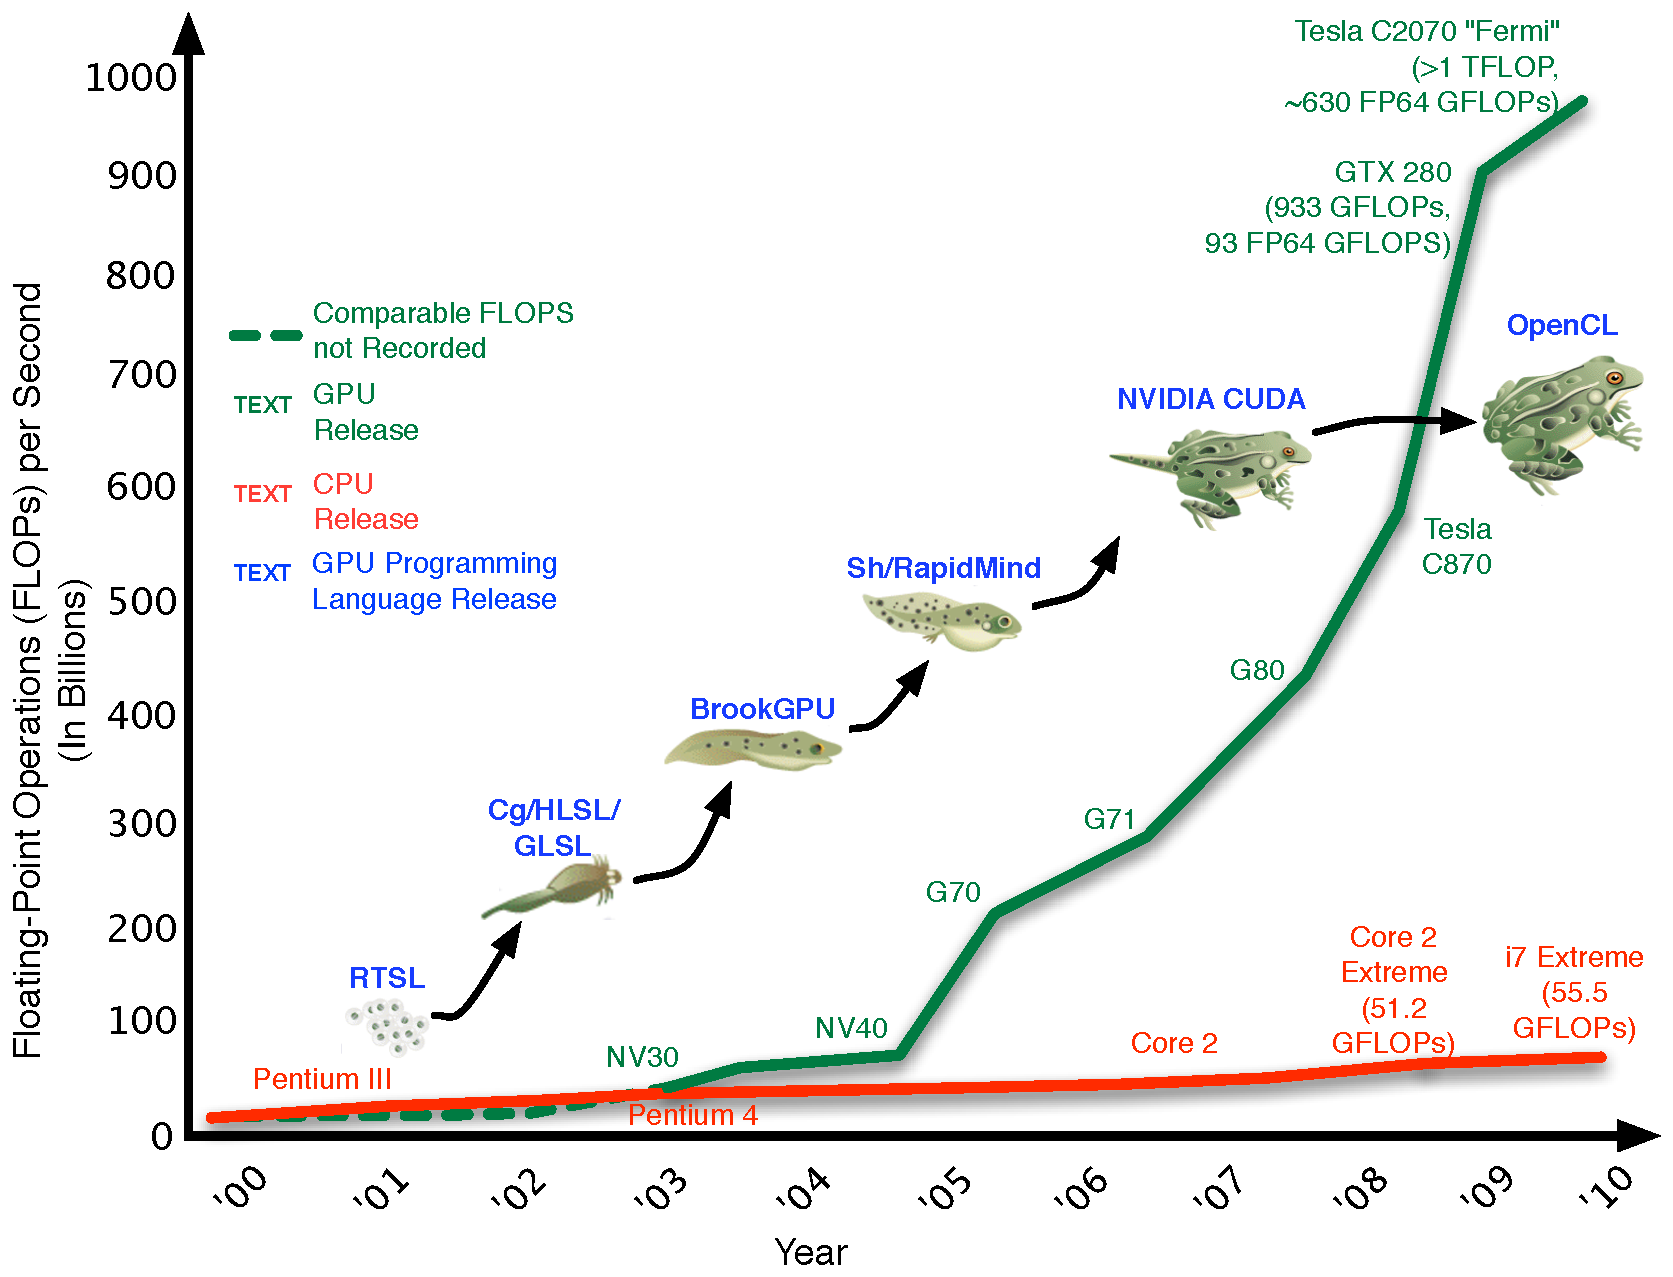
\includegraphics[width=0.6\textwidth]{../figures/prospectus/GPU_Evolution_opencl.pdf}
\caption{Performance comparison for Graphics Processing Units (GPUs). GFLOP/sec data based on \cite{Behr2009, OpenCL2009}. Although data in this figure was last added in 2010, the divide between NVidia and Intel hardware continues to persist today. Currently, the NVidia M2070 (Fermi-class) GPU is capable of 515 GFLOP/sec in double precision, and the NVidia K20 (Kepler-class) GPU is capable of 1.17 TFLOP/sec in double precision \cite{CudaGuide2013}.}
%Meanwhile, the Intel Westmere EP and SandyBridge chips tout 71.8 GFLOP/sec and 157.7 GFLOP/sec respectively, leaving the CPUs an order of magnitude behind NVidia \cite{IntelGFLOPs}}
\label{fig:floating-point-operations-per-second}
\end{figure}

\section{OpenCL}

Due to the success of CUDA (architecture, language, compiler, etc.), and partly because it was vendor specific and closed source, the OpenCL standard for GPU computing was proposed in 2009 \cite{OpenCL2009}. When CUDA was released in 2006, NVidia was not the only contender in the ring of GPU computing: AMD/ATI also had programmable GPUs that could be targeted by a high level language called Brook+ \cite{BrookGPU2004}. Distantly related, Intel was already working toward multi-/many-core architectures that could be targeted by Intel Threaded Building Blocks \cite{IntelTBB}. The OpenCL standard proposed a parallel computing language with the ability to run on any multi-/many-core architecture. The standard is maintained by the Khronos Group, an advisory committee with representatives from the biggest names in hardware and computing (e.g., Apple, AMD, Intel, NVidia, Samsung, Sony, etc.). 

At the onset of this work it was our decision to utilize OpenCL. The GPU computing market was relatively young, and no single company had a dominant share of the HPC market. GPU hardware from both NVidia and ATI was evolving rapidly and OpenCL promised functional portability (i.e., it would run everywhere), so we hedged our bets on the most likely technology to be supported across vendors going into the future. Note that functional portability does not guarantee performance portability (i.e., optimal kernels for NVidia are not optimal for ATI). Some features like 2-D and 3-D textures, which are part of the CUDA standard, are vendor provided extensions in OpenCL and not supported everywhere. 


\subsection{OpenCL Memory and Execution Models}

In Figure~\ref{fig:opencl_execute_model} The OpenCL language \cite{OpenCL2009} assumes a lowest common denominator of hardware capabilities to provide functional portability. 
For example, all target architectures are assumed to support some level of SIMD (Single Instruction Multiple Data) execution for kernels. Multiple \textit{work-items} execute a kernel in parallel. 
A collection of work-items performing the same task is called a \textit{work-group}. While a user might think of work-groups as executing all work-items simultaneously, the work-items are divided at the hardware level into one or more SIMD \textit{warps}, which are executed by a single multiprocessor. For the Fermi and Kepler families of NVidia GPUs, a warp is 32 work-items \cite{CudaGuide2013}. 


\begin{figure}
\centering
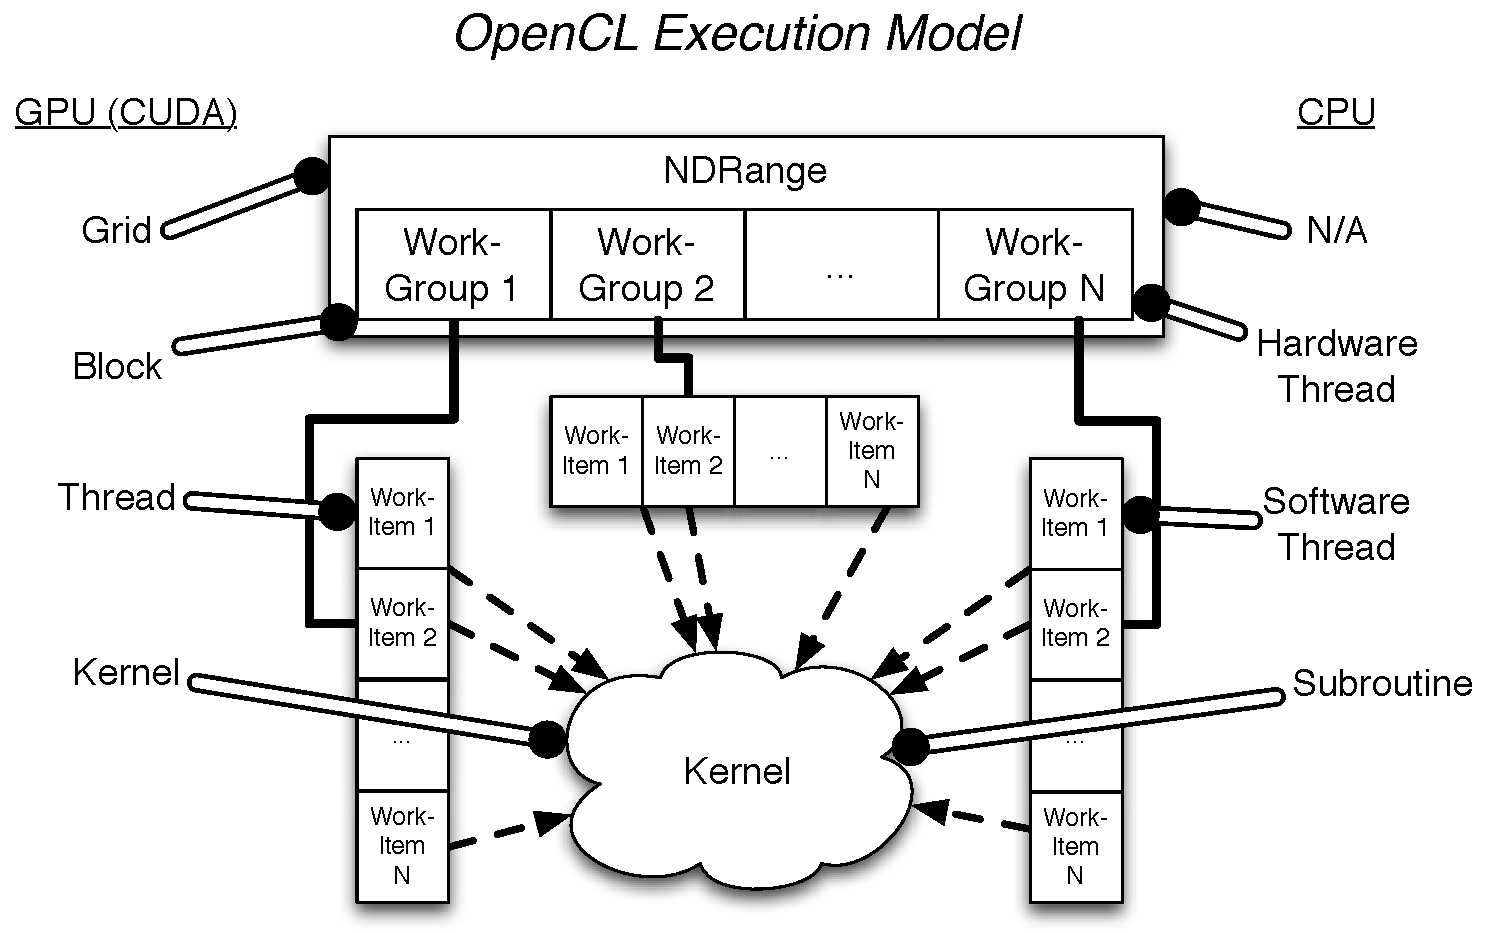
\includegraphics[width=0.6\textwidth]{../figures/prospectus/opencl_execute_model.pdf}
\caption{The OpenCL execution model executes a kernel in parallel across many work-items. A collection of work-items execute in SIMD as a work-group. The work-groups are further bundled into an NDRange representing the full set of tasks executed within a kernel. } 
\label{fig:opencl_execute_model}
\end{figure}

OpenCL assumes a tiered memory hierarchy that provides fast but small \textit{local memory} space that is shared within a work-group \cite{OpenCL2009}. Local memory on Fermi GPUs is 48 KB per multiprocessor \cite{CudaGuide2013}. The \textit{global device memory} allows sharing between work-groups and is the slowest but most abundant memory. 
In the GPU computing literature, the terms \textit{thread} and \textit{shared memory} are synonymous to \textit{work-item} and \textit{local memory} respectively, and are preferred below. 


At the hardware level, a \textit{thread} executes instructions on the GPU. On Fermi level GPUs, groups of 32 threads are referred to as \textit{warps}. A warp is the unit of threads executed concurrently on a single \textit{multi-processor}. 
In OpenCL (i.e., software), a collection of hardware threads performing the same instructions are referred to as a \textit{work-group} of \textit{work-items}. Work-groups execute as a collection of warps constrained to the same multiprocessor. Multiple work-groups of matching dimension are grouped into an \textit{NDRange}. Figure~\ref{fig:grid-of-thread-blocks} shows how threads/work-items are grouped into NDRanges. The \textit{kernel} provides a master set of instructions
for all threads in an NDRange \cite{OpenCL2009}. 


NVidia GPUs have a tiered memory hierarchy related to the grouping of threads described above. 
In multiprocessors, each computing core executes a thread with a limited set of registers. The number of registers varies with the generation of hardware, but always come in small quantities (e.g., 32K shared by all threads of a multiprocessor on the Fermi). Accessing registers is free, but keeping data in registers requires an effort to maintain balance between kernel complexity and the number of threads per block. Threads of a single work-group can share information within a multiprocessor through \textit{shared memory}. With only 48 KB 
available per 
multiprocessor \cite{CudaGuide2011}, shared memory is another fast but limited resource on the GPU. OpenCL refers to shared memory as \textit{local memory}. 
Sharing information across multiprocessors is possible in \textit{global device memory}---the largest and slowest memory space on the GPU. To improve seek times into global memory, Fermi level architectures include L1 on each multiprocessor and a shared L2 cache for all multiprocessors.


Under OpenCL, the equivalent to CUDA local memory is called \textit{private memory} and is also reserved read-only per work-item in global device memory. CUDA's shared memory is labeled \textit{local memory} and shared by threads of a work-group. The CUDA texture and constant caches are known as \textit{Global/Constant Cache}, and similar to CUDA, exist outside of developer control. OpenCL refers to \textit{global memory} and \textit{constant memory} when referring to read/write and read-only sections of CUDA's global device memory (respectively). Finally, CUDA textures are equivalent to OpenCL \textit{buffers} (1-D arrays) or \textit{images} (2-D/3-D arrays) \cite{OpenCL2009}.



\begin{figure}
\centering
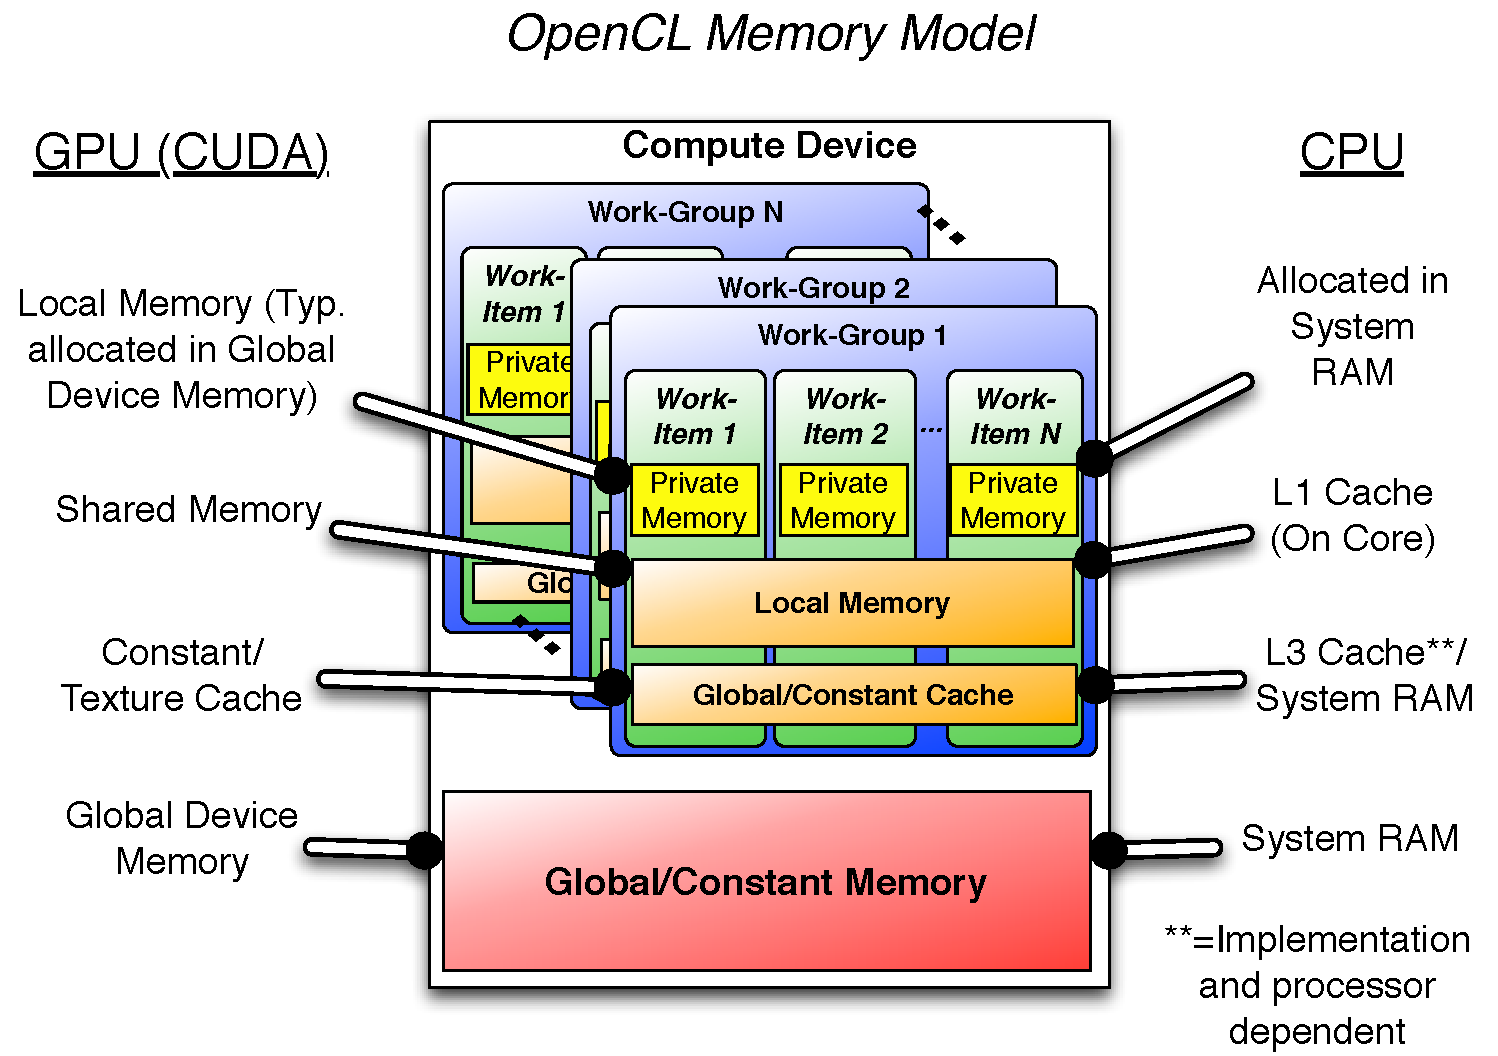
\includegraphics[width=0.6\textwidth]{../figures/prospectus/opencl_memory_model.pdf}
\caption{The OpenCL memory model provides a hierarchy of increasingly faster memories, each with smaller size and more limited scope. A single GPU contains multiple multiprocessors and a large global memory shared by all multiprocessors. Within each multiprocessor, the many cores/threads execute work-items and have access to local and cache memory shared with other work-items of the same multiprocessor. Individual work-items also private memory independent from other work-items. The OpenCL memory model generically abstracts the memory architectures for both CPUs and GPUs.} 
\label{fig:opencl_memory_model}
\end{figure}



\section{Sparse Matrix Support on the GPU}

One thing missing from the original release of CUDA was sparse matrix algebra support. 
This led to investigations like \cite{Bell2009,SuKeutzer2012} and resulted in third party libraries like CUSP \cite{Cusp2012} and ViennaCL \cite{Rupp2010,Rupp2010a}, which are sparse matrix libraries developed for the GPU. The CUSP and ViennaCL libraries are very similar in that they both provide sparse and dense matrix containers, vector containers, iterative Krylov solvers, preconditioners, etc. Both libraries offer similar sparse matrix containers including: Coordinate Matrix format (COO), Compressed-Row Storage format (CSR), ELLPACK Storage format (ELL), and a Hybrid Format (HYB) that is the combination of ELL and CSR. All of these formats were ported to the GPU in \cite{Bell2009} and have also been included in the CUDA SDK since then as part of the cuSPARSE library.  

ViennaCL provides seamless interoperability with the Boost::UBLAS, EIGEN and MTL libraries via C++ templates. We test the performance of our algorithm on one or more CPUs with the Boost::UBLAS library. 

%TODO: get date
NVidia eventually included a library named CUSPARSE as part of the CUDA SDK. Initial releases were 
Developers either implemented their own kernels (as we did in \cite{BolligFlyerErlebacher2012}) or   


%TODO: CUDA MPI not a feature provided by OpenCL. 

Performance of SpMV on GPU will not be optimal. Often one finds in literature examples of applications that have been accelerated by huge factors. In fact, speedup factors greater than 10x should never be possible for SpMV. In order to manage expectations of how much faster tasks will operate on the GPU we can turn to a \emph{roofline model} \cite{Williams2009}. The roofline model 


Most recently, the PETSc library gained GPU support with the addition of both CUSP \cite{Cusp2012} and ViennCL \cite{Rupp2010} back-ends \cite{Minden2010}. PETSc---which dates back to the early 1990s---is widely-used for solving PDEs with proven scalability on the world's top supercomputers. PETSc provides distributed sparse and dense matrix algebra, Krylov solvers, and preconditioners. The support for GPU back-ends allows a vast number of applications that have been developed over more than two decades to run on multiple GPUs with minimal modification. Since PETSc already has overlapping MPI communication and computation for distributed CPU environments, the GPU offloaded applications also benefit from this feature. Yokota et al. \cite{YokotaGPU2010} demonstrate that PETSc multi-GPU applications can scale excellently (in the strong sense) when configured for tree-based communication, which arises naturally from Fast Multipole Methods. The authors scale their boundary element method across 256 GPUs (2 per compute node) with 80\% parallel efficiency, and 512 GPUs (4 per compute node) with 50\% efficiency. In contrast to this our distributed implementation currently achieves no more than 57\% parallel efficiency when spanning 8 GPUs. While we do not take advantage of tree-based communications, this is planned as part of the future work to improve scalability. 





%TODO verify date of open source
In 2012 NVidia open sourced CUDA to lower level virtual machines. This opened the possibility of directly compiling other languages like Python (Anaconda) to build kernels directly within the Python language for CUDA. 

GPUs currently support single and double precision. RBF-FD certainly requires double precision at the moment. Solving for the weights in single precision might work, but the lower precision would not be able to handle the ill-conditioned system. Projecting double precision weights into single precision results in weights that sum to $\approx 10^{-4}$, a poor approximation to zero. 
%
%the addition of a new software layer that finally made GPGPU accessible to the general public. The CUDA API includes routines for memory control, interoperability with graphics contexts (i.e., 
%OpenGL programs), and provides GPU implementation subsets of BLAS and FFTW libraries \cite{CudaGuide2013}. After the undeniable success of CUDA for C, new projects emerged to encourage GPU programming in languages like FORTRAN (see e.g., HMPP \cite{HMPP2009} and Portland Group Inc.'s CUDA-FORTRAN \cite{CudaFortran2009}). 
%
%This transition was 
%followed closely by evolving programming languages. Today, GPUs can be leveraged from C/C++, FORTRAN, Java, Python, MATLAB, and more. The list seems endless, with new developments appearing every day. 



%\section{Test Environments}
%
%\begin{itemize}	
%\item Early testing was completed on the Keeneland GPU cluster. At the time Keeneland was in the Keeneland Initial Deployment System (KIDS) had 320 NVidia M2070 GPUs (Fermi). 240 CPUs. 6GB of memory. 
%%\item The Spear cluster at FSU has 16x NVIDIA Tesla m2050 GPUs. 3GB of memory. 
%\item The Cascade cluster at the Minnesota Supercomputing Institute (UMN) has 32x NVidia M2070 GPUs. 8 nodes, 12 cores each with four GPUs attached to each. 6GB of memory each. In addition, Cascade has 8 NVidia Kepler K20 GPUs. 
%\end{itemize}

\section{Managing Expectations for the GPU}
\begin{figure} 
\begin{subfigure}{0.45\textwidth}
\centering
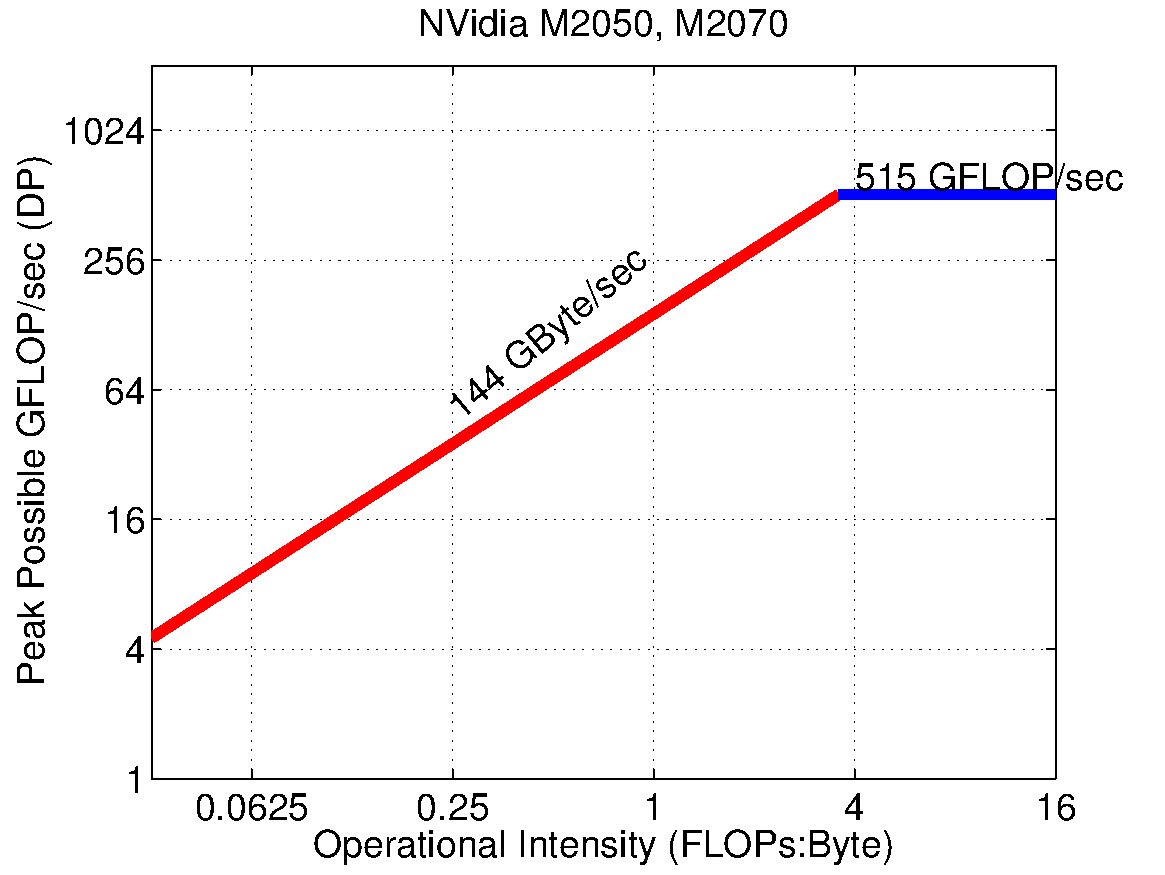
\includegraphics[width=\textwidth]{../figures/spmv/roofline_m2050_m2070-eps-converted-to.pdf}
\caption{Roofline Model for NVidia Fermi class GPUs, M2050 and M2070. SpMV Peak: 18.5 GFLOP/sec (double precision).}
\label{fig:roofline_m2070}
\end{subfigure}
\quad
\begin{subfigure}{0.45\textwidth}
\centering
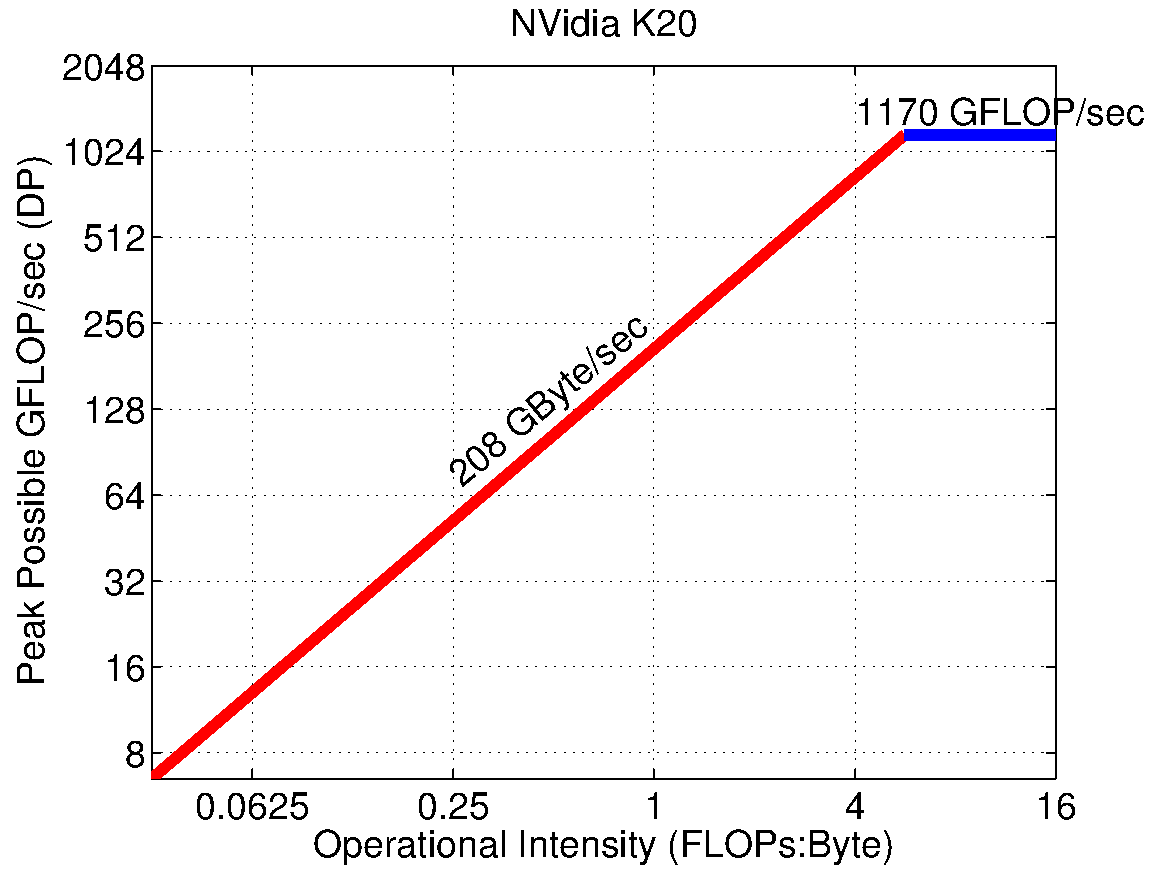
\includegraphics[width=\textwidth]{../figures/spmv/roofline_k20-eps-converted-to.pdf}
\caption{Roofline Model for NVidia Kepler K20. SpMV Peak: 26 GFLOP/sec (double precision).}
\label{fig:roofline_k20}
\end{subfigure}
\caption{Roofline models manage expectations for maximum possible GFLOP/sec based on the Operational Intensity of kernels. The SpMV needed by RBF-FD has an operational intensity of $0.25$. }
\end{figure}


Success stories abound on the GPU citing massive gains in performance. However, many like \cite{Phillips2009} appear to be impossible

RBF-FD is embarrassingly parallel with stencils applied independently. Unfortunately, maximum concurrency does not always imply perfect performance. %TODO: (SHOW RBF-FD benchmarks for Vortex and Cosine as an example of 1x and 2x SpMV on GPU; state that the generation GPU they were run on has a peak of xxx which means performance was xxx\% (dismal).).

On the Fermi GPUs (Figure~\ref{fig:roofline_m2070}) at 144 GB/s you need an OI of 4 to reach the peak of 515 GFLOP/sec per card. On the K20 (Figure~\ref{fig:roofline_k20}) you need 6 to hit the peak 1.17 TFLOP/s (208 GB/s). But with an OI of 1/16 you could get 9 GFLOP/sec on the Fermi and 13 on the K20 (compared to the 2 GFLOP/sec on Itasca). 

%
%\begin{verbatim}
%"__kernel void vec_mul(\n"
%"          __global const unsigned int * row_indices,\n"
%"          __global const unsigned int * column_indices, \n"
%"          __global const float * elements,\n"
%"          __global const float * vector,  \n"
%"          __global float * result,\n"
%"          unsigned int size) \n"
%"{ \n"
%"  for (unsigned int row = get_global_id(0); row < size; row += get_global_size(0))\n"
%"  {\n"
%"    float dot_prod = 0.0f;\n"
%"    unsigned int row_end = row_indices[row+1];\n"
%"    for (unsigned int i = row_indices[row]; i < row_end; ++i)\n"
%"      dot_prod += elements[i] * vector[column_indices[i]];\n"
%"    result[row] = dot_prod;\n"
%"  }\n"
%"}\n"
%\end{verbatim}
%
%\begin{verbatim}
%"__kernel void vec_mul(\n"
%"    const __global int* coords,\n"
%"    const __global float* elements,\n"
%"    const __global const float * vector,\n"
%"    __global float * result,\n"
%"    const unsigned int row_num,\n"
%"    const unsigned int col_num,\n"
%"    const unsigned int internal_row_num,\n"
%"    const unsigned int items_per_row,\n"
%"    const unsigned int aligned_items_per_row\n"
%"    )\n"
%"{\n"
%"    uint glb_id = get_global_id(0);\n"
%"    uint glb_sz = get_global_size(0);\n"
%"    for(uint row_id = glb_id; row_id < row_num; row_id += glb_sz)\n"
%"    {\n"
%"        float sum = 0;\n"
%"        \n"
%"        uint offset = row_id;\n"
%"        for(uint item_id = 0; item_id < items_per_row; item_id++, offset += internal_row_num)\n"
%"        {\n"
%"            float val = elements[offset];\n"
%"            if(val != 0.0f)\n"
%"            {\n"
%"                int col = coords[offset];    \n"
%"                sum += (vector[col] * val);\n"
%"            }\n"
%"            \n"
%"        }\n"
%"        result[row_id] = sum;\n"
%"    }\n"
%"}\n"
%\end{verbatim}


%TODO: targeting the GPU for SpMV (how to write a kernel as forloop without the for)

 
%TODO: list all known work on SpMV for GPU
%TODO: emphasize that the GPU SpMV has been studied since before 2006.
%TODO: SpMV condenses sparse matrix to dense form. 
%TODO: each of the dense forms are unique (describe each)
%TODO: newer forms are available




%TODO: ALL SPMV related work.
%\cite{Bell2009} 
%TODO: \cite{Kreuzer2012} in distributed GPU. 
%\cite{Vuduc2005} etc. 



In our initial implementation, published in \cite{BolligFlyerErlebacher2012}, all bets were hedged in favor of OpenCL as the future of GPU computing. Custom kernels were developed to apply RBF-FD weights in the equivalent of a CSR SpMV. 


\section{Performance}
\subsection{GFLOP/sec}
In order to quantify the performance of our implementation, we can measure two
factors. First, we can check the speedup achieved on the GPU relative to the
CPU to get an idea of how much return of investment is to be expected by all
the effort in porting the application to the GPU. Speedup is measured as the
time to execute on the CPU divided by the time to execute on the GPU. 

The second quantification is to check the throughput of the process. By
quantifying the GFLOP throughput we have a measure that tells us two things:
first, a concrete number quantifying the amount of work performed per second by
either hardware, and second because we can calculate the peak throughput possible on
each hardware, we also have a measure of how occupied our CPU/GPU units are.
With the GFLOP/sec we can also determine the cost per watt for computation and
conclude on what problem sizes the GPU is cost effective to target and use. 

Now, as we parallelize across multiple GPUs, these same numbers can come into
play. However we are also interested in the efficiency. Efficiency is the
speedup divided by the number of processors. With efficiency we have a measure
of how well-utilized processors are as we scale either the problem size (weak)
or the number of processors (strong). As the efficiency diminishes we can
conclude on how many stencils/nodes per processor will keep our processors
occupied balanced with the shortest compute time possible (i.e., we are
maximizing return of investment). 

\subsection{Expectations in Performance}
Many GPU applications claim a 50x or higher speedup. This will never be the case for RBF-FD for the simple reason that the method reduces to an SpMV. The SpMV is a low computational complexity operation with only two operations for every one memory load. 




\subsection{OpenCL vs CUDA}
The market is volatile. Companies survive by investing margins in their next great product. If a product fails or the company faces a recall, their survival may come into question. Thus far, NVidia's CUDA has been wildly popular, but for the longest time (until May 2012) it was closed source. The closed source limited the language to NVidia hardware. As such, the OpenCL language gained popularity due to its support for AMD, Intel, mobile devices, web browsers, etc. NVidia's push to provide an open source compiler may be an attempt to regain the market share, but OpenCL appears to be on good footing. One other point: with an open source NVidia compiler, OpenCL can be optimized by the more mature NVidia compiler for their proprietary hardware. OpenCL compilers are also becoming more sophisticated at auto-optimization. 


\subsection{Custom Kernels}
\label{sec:custom_gpu_kernels}

From the definition of RBF-FD we can formulate the problem computationally in two ways. First, stencil operations are independent. Therefore, we can write kernels with perfect parallelism by dedicating a single thread per stencil or a group of threads per stencil.  

Unfortunately, perfect concurrency does not imply perfect or even ideal concurrency on the GPU. 

Since our focus within this work is to lay the foundation for parallel computing
with RBF-FD, we have made several simplifying assumptions in our code design.
Libraries like PETsc, Hypre, Trilinos and Deal.ii distribute sparse matrix
operations in similar fashion to our approach. When work initially began on this
dissertation, none of these competing libraries contained support for the GPU.
PETsc is currently developing support for the GPU, but we have not had the
chance to consider it yet. 

Our codebase began as a prototype demonstrating the feasibility of RBF-FD
operating on the GPU. The initial code, published in \cite{BolligFlyerErlebacher2012}, was developed as $N$ independent dot
products of weights and solution values to approximate derivatives. Weights were
stored linearly in memory, with the solution values read randomly. On the GPU,
stencils were evaluated independently by threads, or shared by a warp of
threads. Operating on stencils in this way implied that GPU kernels were to be
hand written, tuned and optimized. 

Much later, our perspective evolved to see derivative approximation and
time-stepping as sparse matrix operations. This opened new possibilities for
optimization and allowed us to forego hand optimization and fine-tuning of GPU
kernels. With all of the effort put into optimizing sparse operations within
libraries like CUSP \cite{Bell2009}, ViennaCL \cite{Rupp2010} and even the
NVidia provided CUSPARSE \cite{CudaToolkitDoc}, formulating the problem in terms of
sparse matrix operations allows us to quickly prototype on the GPU and leverage
all of the optimizations available within the third party libraries. 


\subsection{Explicit Solvers}

%TODO: add explicit equation formula

Our initial implementation in \cite{BolligFlyerErlebacher2012} leverages the GPU for acceleration of the standard fourth order Runge-Kutta (RK4) scheme. Stencil weights are calculated once at the beginning of the simulation, and reused in every iteration. Subsequent runs load weights from disk. Ignoring code initialization, the cost of the algorithm is simply the explicit time advancement of the solution. 

Figure~\ref{fig:multi_GPU_flow} summarizes the time advancement steps for the multi-CPU/GPU implementation. The RK4 steps are: 
\begin{eqnarray} 
\mathbf{k}_1 &=& \Delta t f(t_n, \mathbf{u}_n) \nonumber \\
\mathbf{k}_2 &=& \Delta t f(t_n+\frac{1}{2}\Delta t, \mathbf{u}_n + \frac{1}{2}\mathbf{k}_1) \nonumber \\
\mathbf{k}_3 &=& \Delta t f(t_n+\frac{1}{2}\Delta t, \mathbf{u}_n + \frac{1}{2}\mathbf{k}_2)  \label{eqn:rk4}\\
\mathbf{k}_4 &=& \Delta t f(t_n+\Delta t, \mathbf{u}_n + \mathbf{k}_3) \nonumber \\
\mathbf{u}_{n+1} &=& \mathbf{u}_{n} + \frac{1}{6}(\mathbf{k}_1 + 2\mathbf{k}_2 + 2\mathbf{k}_3 +\mathbf{k}_4), \nonumber
\end{eqnarray}
where each equation has a corresponding kernel launch. To handle a variety of Runga-Kutta implementations, steps $\mathbf{k}_{1\rightarrow4}$ correspond to calls to the same kernel with different arguments. The evaluation kernel returns two output vectors: 
\begin{enumerate} 
\item $\mathbf{k}_i = \Delta t f(t_n + \alpha_{i} \Delta t, \mathbf{u}_n + \alpha_{i} \mathbf{k}_{i-1})$, for steps $i=1,2,3,4$, and
\item  $\mathbf{u}_n + \alpha_{i+1} \mathbf{k}_i$
\end{enumerate} 
We choose $\alpha_{i}=0, \frac{1}{2}, \frac{1}{2}, 1, 0$ and $\mathbf{k}_{0} = \mathbf{u}_n$. The second output for each $\mathbf{k}_{i=1,2,3}$ serves as input to the next evaluation, $\mathbf{k}_{i+1}$. In an effort to avoid an extra kernel launch---and corresponding memory loads---the SAXPY that produces the second output uses the same evaluation kernel. Both outputs are stored in global device memory. When the computation spans multiple GPUs, steps $\mathbf{k}_{1\rightarrow3}$ are each followed by a communication barrier to synchronize the subsets $\mathcal{O}$ and $\mathcal{R}$ of the second output (this includes copying the subsets between GPU and CPU). An additional synchronization occurs on the updated solution, $\mathbf{u}_{n+1}$, to ensure that all GPUs share a consistent view of the solution going into the next time-step.

\begin{figure}[t]
      \centering
       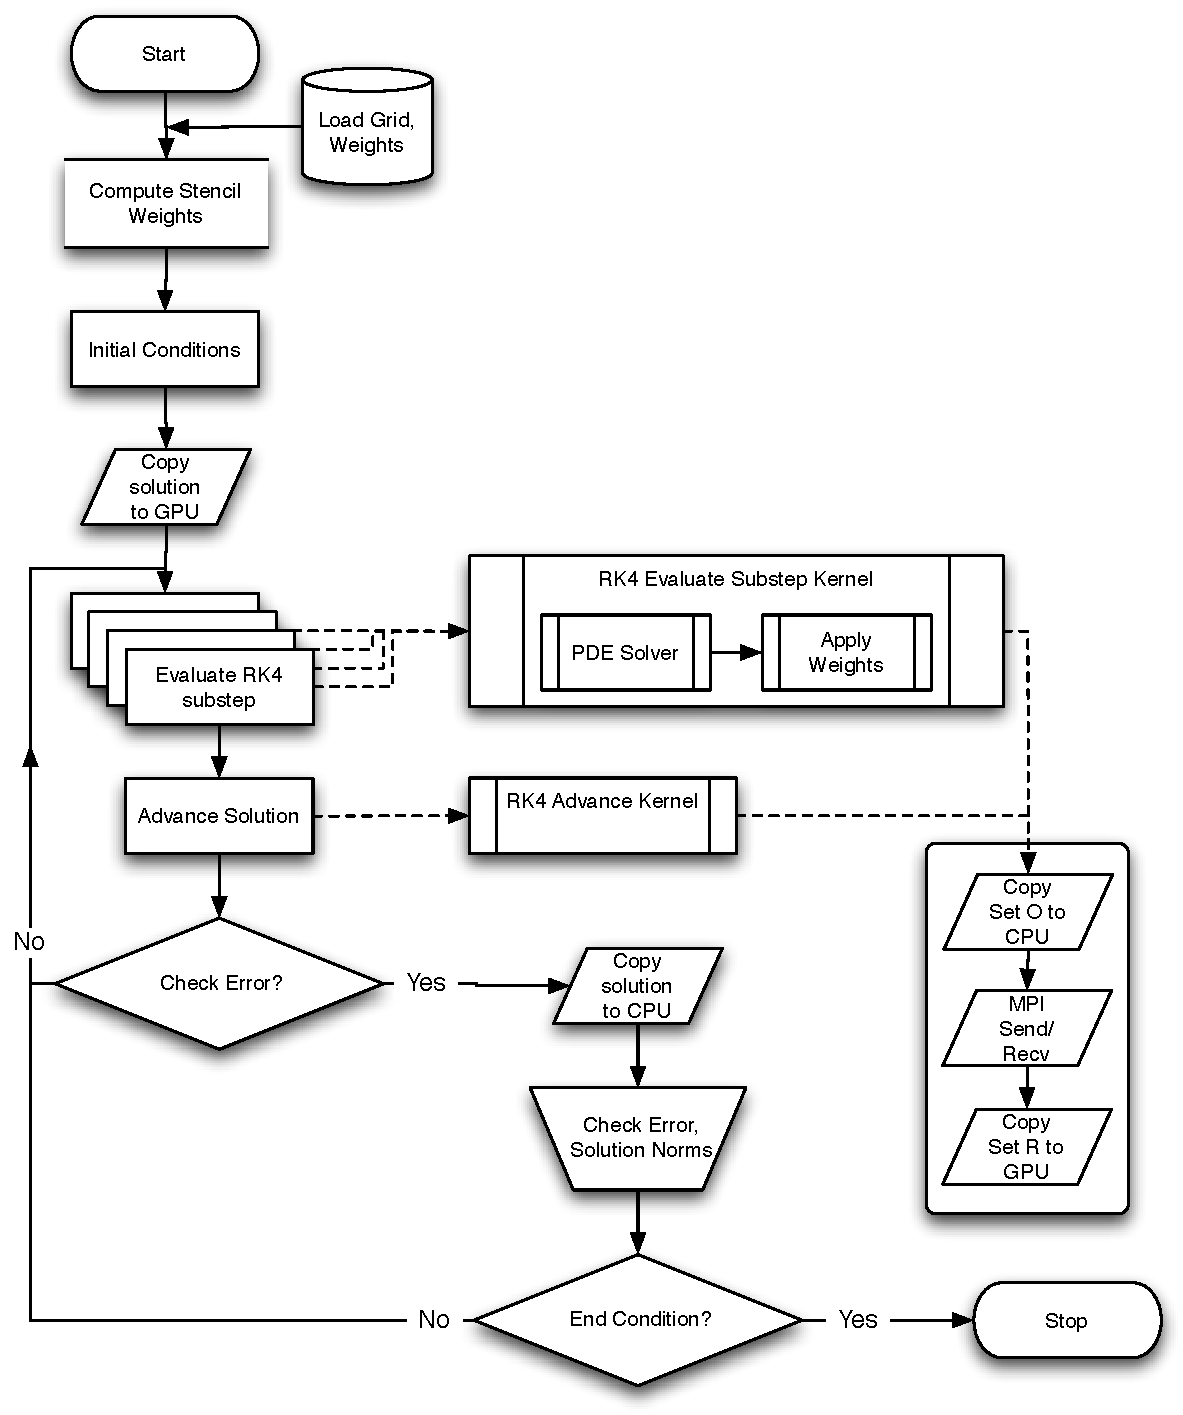
\includegraphics[width=5in]{../figures/paper1/figures/omnigraffle/RK4_multi_GPU_flow.pdf}
      \caption{Workflow for RK4 on multiple GPUs. }
      \label{fig:multi_GPU_flow}
\end{figure}


To evaluate $\mathbf{k}_{1\rightarrow4}$ in Equation~\ref{eqn:rk4}, the discretized operators from Equation~(\ref{eq:evaluation_with_hyperviscosity}) are applied using sparse matrix-vector multiplication. If the operator $D$ is composed of multiple derivatives, a differentiation matrix for each derivative is applied independently, including an additional multiplication for the discretized $H$ operator.
 On the GPU, the kernel parallelizes across rows of the DMs, so all derivatives for stencils are computed in one kernel call.


For the GPU, the OpenCL language \cite{OpenCL2009} assumes a lowest common denominator of hardware capabilities to provide functional portability. For example, all target architectures are assumed to support some level of SIMD (Single Instruction Multiple Data) execution for kernels. Multiple \textit{work-items} execute a kernel in parallel. 
A collection of work-items performing the same task is called a \textit{work-group}. While a user might think of work-groups as executing all work-items simultaneously, the work-items are divided at the hardware level into one or more SIMD \textit{warps}, which are executed by a single multiprocessor. On the family of Fermi GPUs, a warp is 32 work-items \cite{CudaGuide2011}. 
OpenCL assumes a tiered memory hierarchy that provides fast but small \textit{local memory} space that is shared within a work-group \cite{OpenCL2009}. Local memory on Fermi GPUs is 48 KB per multiprocessor \cite{CudaGuide2011}. The \textit{global device memory} allows sharing between work-groups and is the slowest but most abundant memory. 
In the GPU computing literature, the terms \textit{thread} and \textit{shared memory} are synonymous to \textit{work-item} and \textit{local memory} respectively, and are preferred below. 

%Although the primary focus of this paper is the implementation 
%and verification of the RBF-FD method across multiple CPUs and GPUs, 
%we have nonetheless tested two approaches to the computation of derivatives 
Our initial implementation of RBF-FD on multiple GPUs (\cite{BolligFlyerErlebacher2012}) tested two approaches to computation of derivatives. 
%assess the potential for further improvements in performance. 
In both cases, the stencil weights are stored in CSR format \cite{Bell2009}, 
a packed one-dimensional array in global memory with all the weights 
of a single stencil in consecutive memory addresses. Each operator is stored as an independent CSR matrix. The consecutive ordering on the weights implies that the solution vector %structured according to the ordering of set $\mathcal{G}$ 
is treated as random access. 

All the computation on the GPU is performed in 8-byte double precision. 




\subsubsection{Naive Approach: One thread per stencil}

In this first implementation, each thread computes 
the derivative at one stencil center  (Figure~\ref{fig:oneThreadPerStencil}). 
The advantage of this approach is trivial concurrency.  Since each stencil has the same number of neighbors, each derivative has an identical number of computations. As long as the number of stencils is a multiple of the warp size, there are no idle threads. Should the total number of stencils be less than a multiple of the warp size, the final warp would contain idle threads, but the impact on efficiency would be minimal assuming the stencil size is sufficiently large. 

Perfect concurrency from a logical point of view does not 
imply perfect efficiency in practice. 
Unfortunately, the naive approach 
is memory bound. When threads access weights in global memory, 
a full warp accesses a 128-byte segment in a single memory operation \cite{CudaGuide2011}.
Since each thread handles a single stencil, the various threads in a warp access data in very disparate areas of global memory, rather than the same segment. This leads to very large slowdowns as extra memory operations are added for each 128-byte segment that the threads of a warp must access.
However, with stencils sharing many common nodes, and the Fermi hardware providing caching, some weights in the unused portions of the segments might remain in cache long enough to hide the cost of so many additional memory loads. 



\begin{figure}[htbp]
      \centering
       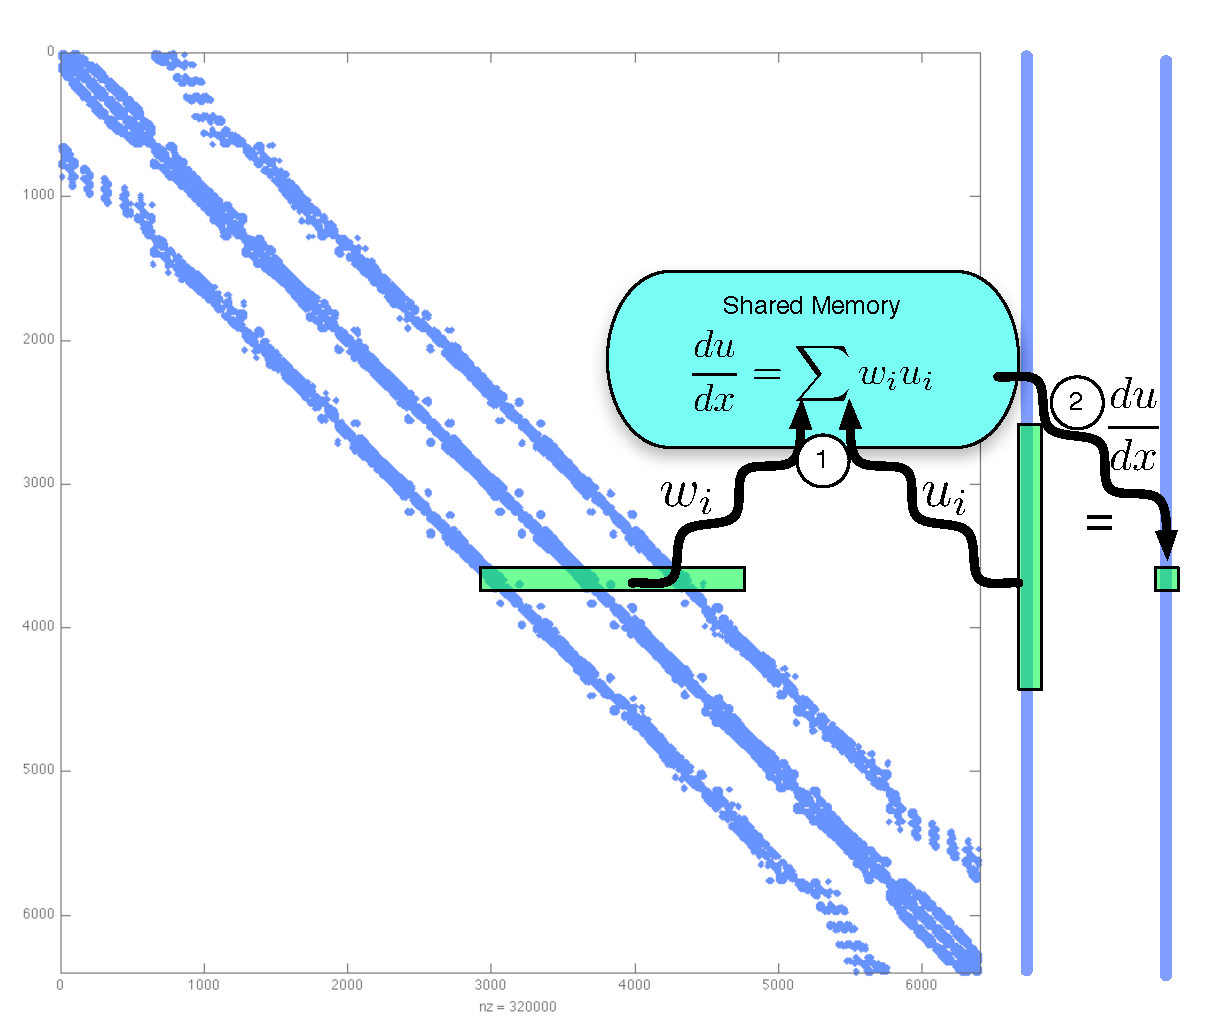
\includegraphics[width=3in]{../figures/paper1/figures/omnigraffle/oneThreadPerStencil.pdf}
      \caption{Naive approach to sparse matrix-vector multiply. Each thread is responsible for the sparse vector dot product of weights and solution values for derivatives at a single stencil.  }
      \label{fig:oneThreadPerStencil}
\end{figure}


\subsubsection{Alternate Approach: One warp per stencil} 

\begin{figure}[htbp]
      \centering
       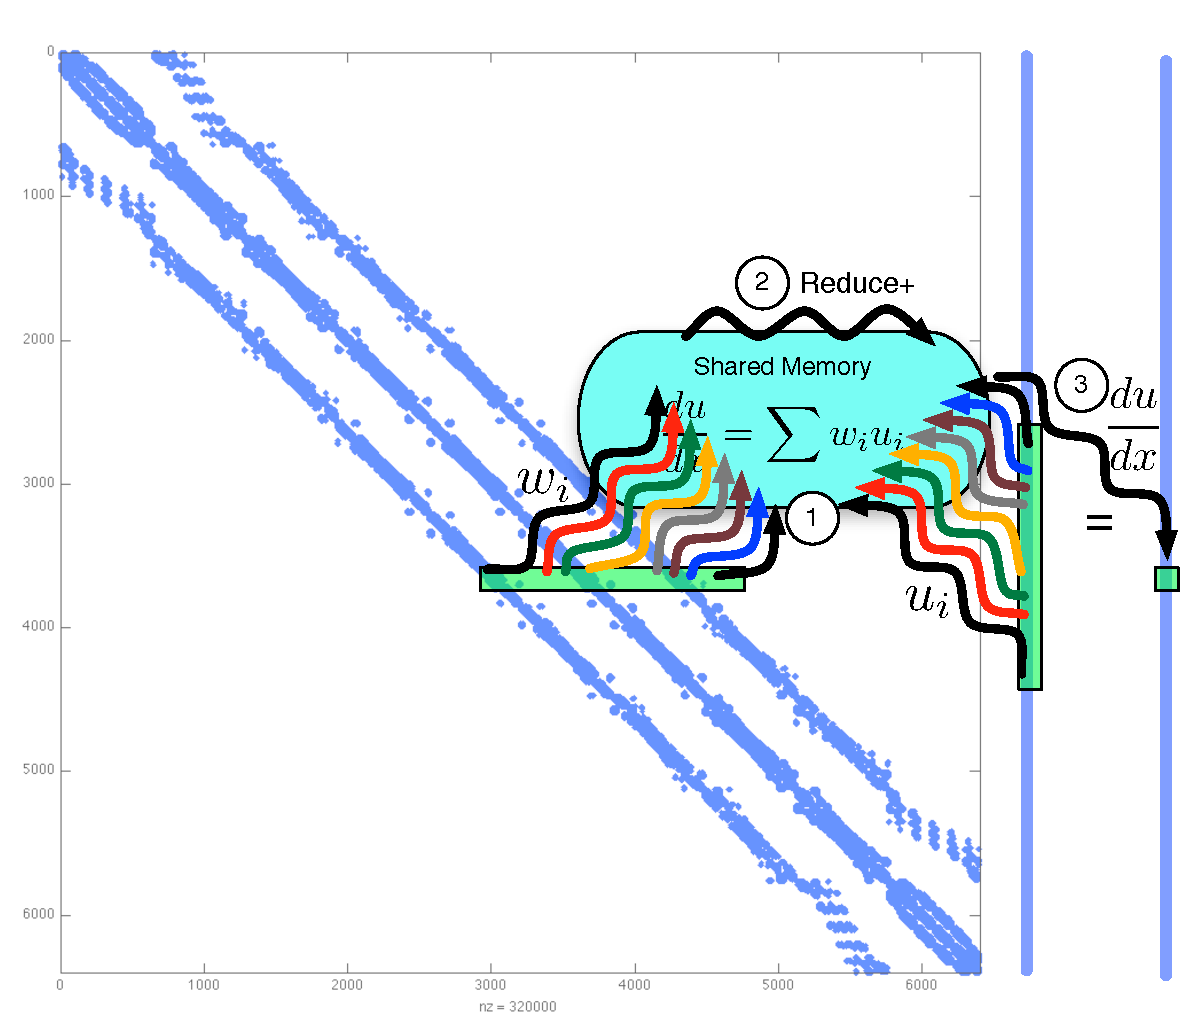
\includegraphics[width=3in]{../figures/paper1/figures/omnigraffle/oneWarpPerStencil.pdf}
      \caption{Alternative approach. A full warp (32 threads) collaborate to apply weights  and compute the derivative at a stencil center. }
      \label{fig:oneWarpPerStencil}
\end{figure}


An alternate approach, illustrated in Figure~\ref{fig:oneWarpPerStencil}, dedicates a full warp of threads to a single stencil. Here, 32 threads load the weights of a stencil and the corresponding elements of the solution vector. As the 32 threads each perform a subset of the dot product, their intermediate sums are accumulated in 32 elements of shared memory (one per thread).
Should  a stencil be larger than the warp size, the warp iterates over the stencil in increments of the warp size until the full dot product is complete. Finally, the first thread of the warp performs a sum reduction across the 32 (warp size)  intermediate sums stored in shared memory and writes the derivative value to global memory. 

By operating on a warp by warp basis, weights for a single stencil are loaded with a reduced number of memory accesses. Memory loads for the solution vector remain random access but see some benefit when solution values for a stencil are in a small neighborhood in the memory space. Proximity in memory can be controlled by node indexing (see Chapter~\ref{chap:stencils}). 

For stencil sizes smaller than 32, some threads in the warp always remain idle. Idle threads do not slow down the computation within a warp, but under-utilization of the GPU is not desirable. For small stencil sizes, caching on the Fermi can hide some of the cost of memory loads for the naive approach, with no idle threads, making it more efficient. The real strength of one warp per stencil is seen for large stencil sizes. 
As part of future work on optimization, we will consider a parallel reduction in shared memory, as well as assigning multiple stencils to a single warp for small  $n$. 





\subsection{ViennaCL} 

In the time since the publication of \cite{BolligFlyerErlebacher2012} custom OpenCL kernels have been dropped in favor of a library called ViennaCL. 

Sparse formats supported by ViennaCL are shown in Figure~\ref{fig:sparse_format}.

\begin{figure}
\centering
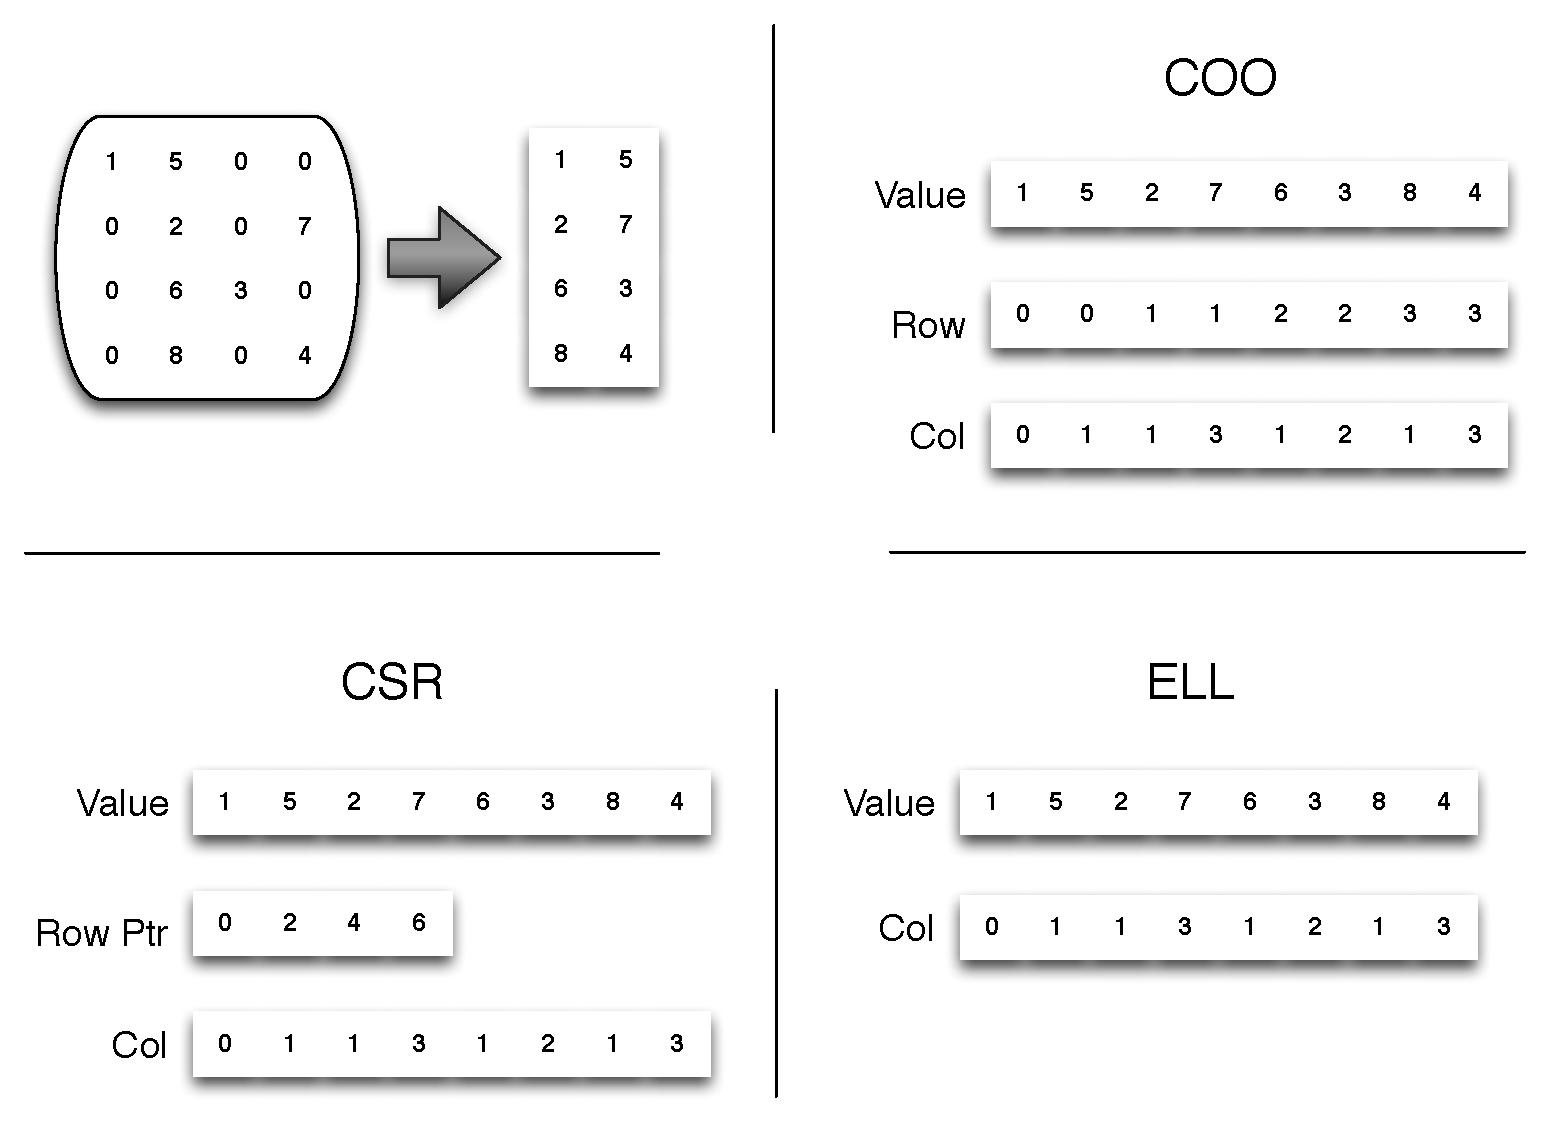
\includegraphics[width=0.9\textwidth]{gpu_content/omnigraffle/SparseStorage.pdf}
\caption{Sparse format example demonstrating a sparse matrix and corresponding storage data structures. ELL format assumes two non-zeros per row. }
\label{fig:sparse_format}
\end{figure}

Other formats exist such as the Hybrid ELL plus CSR (HYB) format \cite{Bell2009}, Diagonal (DIAG) and Jagged Diagonal (JAD) variants, and a number of variants on the ELL format that operate in blocks (BELL), slices (SELL), or both (SBELL) \cite{SuKeutzer2012}. The HYB format stores the bulk of a matrix in an ELL container and the excess non-zeros per row in a CSR format. HYB benefits from reduced storage and memory loads in the ELL, and maintains the generality of a CSR matrix. 

%\begin{figure}
%\centering
%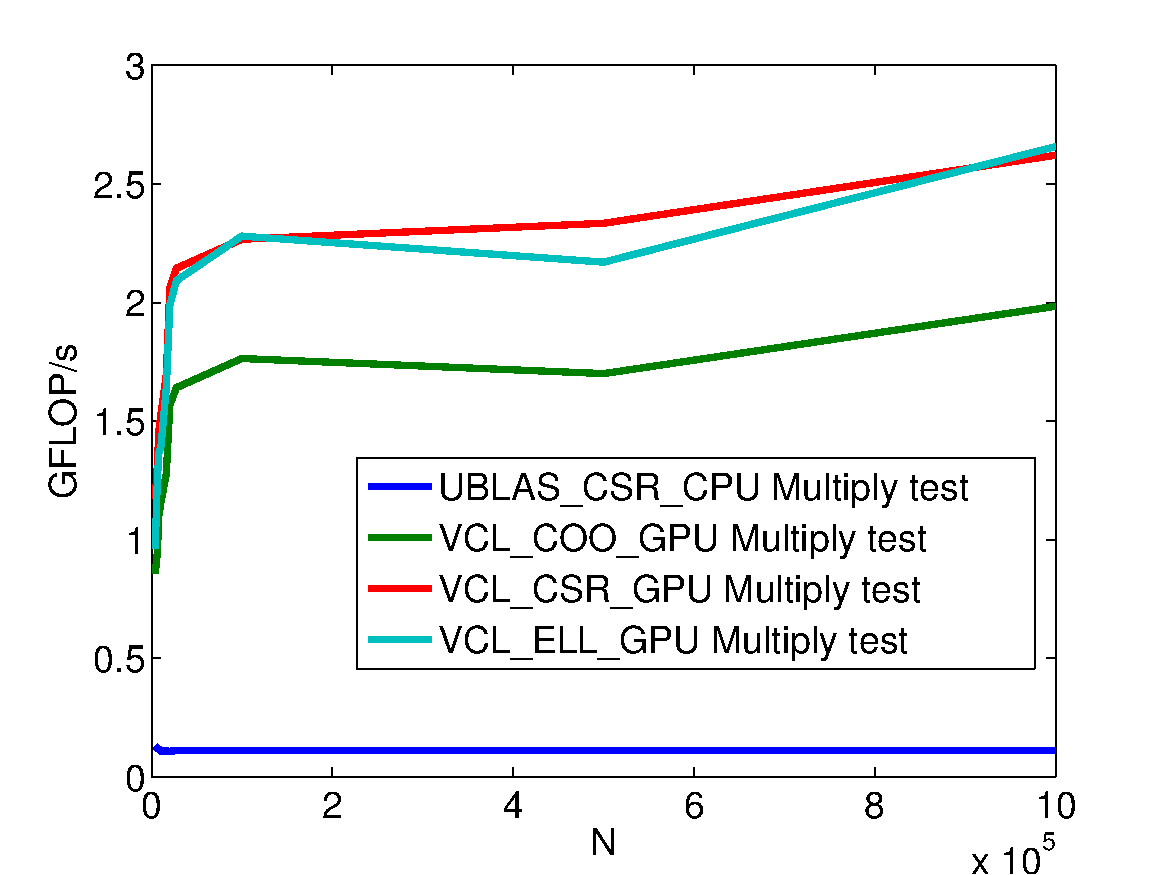
\includegraphics[width=0.5\textwidth]{../figures/spmv/spmv_vcl_gflops-eps-converted-to.pdf}
%\caption{Single GPU ViennaCL SpMV throughput (GFLOP/sec) compared to Boost::uBLAS CSR. Stencil size $n=50$ for all cases.}
%\label{fig:spmv_vcl_gflops}
%\end{figure}

GFLOP/sec calculated as: 
\begin{align}
GFLOP/sec = ^{N * n * 2} /_{t_ms} * 10^{-9}. 
\end{align}



%TODO: paralution
Paralution is another library that provides sparse matrix containers, iterative solvers, preconditioners, etc. Paralution provides interfaces to plug into Deal.ii, OpenFOAM, and other packages, and runs on multi-core CPUs and GPUs. 


To further optimize RBF-FD on the GPU, we formulate the problem in terms of a Sparse Matrix-Vector Mulitply (SpMV). When we consider the problem in this light we generate a single Differentiation Matrix that can see two optimizations not possible with our stencil-based view: 
\begin{itemize} 
\item First, the sparse containers used in SpMV allow for their own unique optimizations to compress storage and leverage hardware cache.
\item Evaluation of multiple derivatives can be accumulated by association into one matrix operation. This reduces the total number of floating point operations required per iteration. 
\end{itemize}


%TODO: tell the story of ViennaCL. 
%TODO: what motivated the switch
The library includes a variety of sparse matrix formats, solvers, preconditioners, etc. Dense and sparse containers simplify targeting the GPU. 

At the onset of work with ViennaCL two things were apparent: 1) the library was incredibly powerful but limited to square matrices; and 2) the library had no support for distributed computing. Our implementation of RBF-FD (\cite{BolligRBFFDCode}) required rectangular matrices resulting from domain decomposition. The enhancements to the API have since been added to the main branch of ViennaCL. 


%TODO: CSR Bytes:Flop ratio: \url{http://arxiv.org/pdf/1101.0091v1.pdf}





%TODO: list example loops for sparse kernels


Due to the assumption that all stencils have equal size, the ELL format is preferred as the default. 
 

\section{Cascade}

The actual observed GFLOP/sec achieved on Cascade's M2070 GPUs with the ViennaCL package is shown in Figure~\ref{fig:gflops_cascade_m2070}. Figure~\ref{fig:gflops_cascade_k20} provides achieved GFLOP/sec for Cascade's K20 GPUs.  

\begin{figure} 
\centering
\begin{subfigure}[t]{0.48\textwidth}
\centering
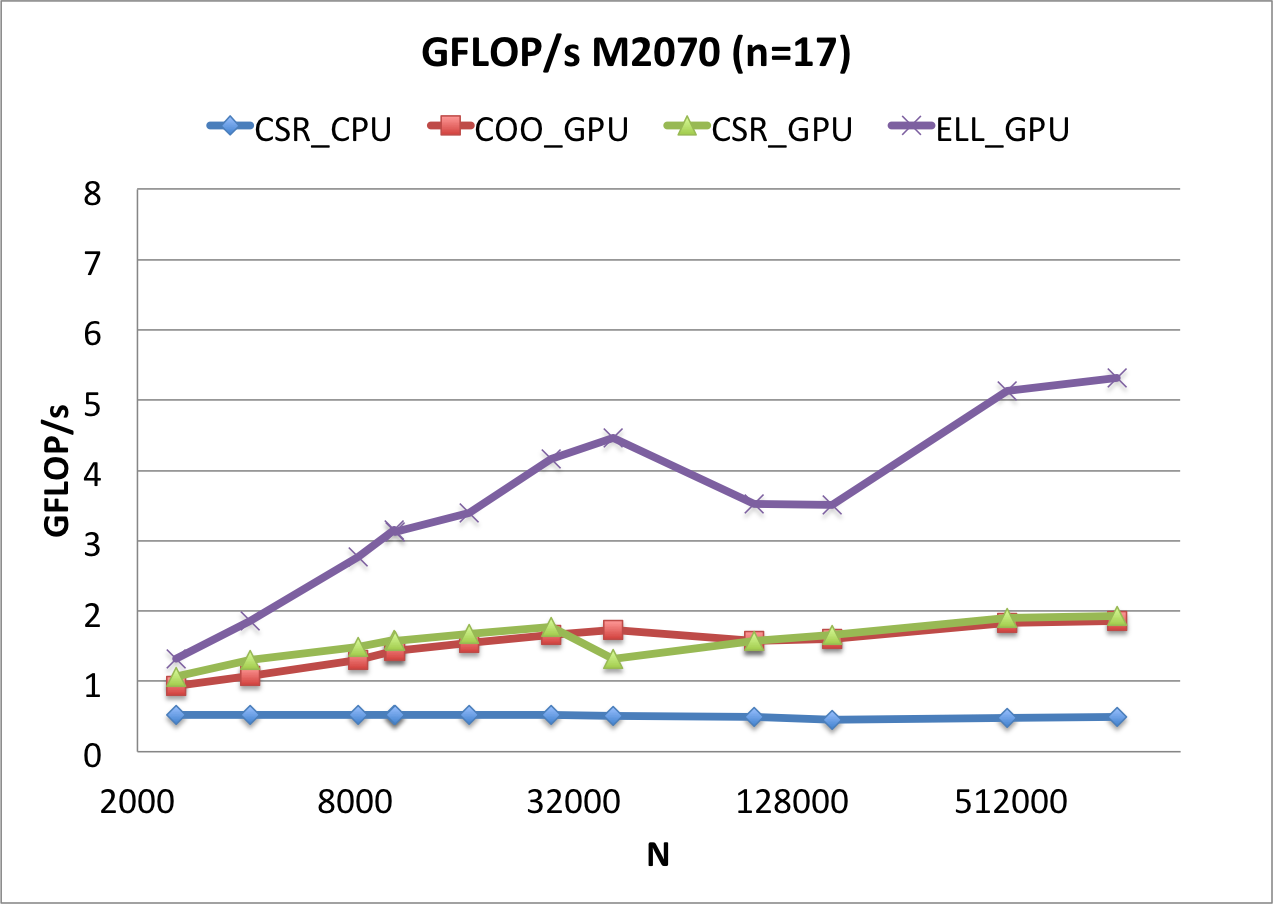
\includegraphics[width=\textwidth]{gpu_content/cascade_spmv/gflops_cascade_m2070_n17.png}
\caption{Stencil size $n=17$}
%\label{fig:gflops_cascade_m2070_n17}
\end{subfigure}
\quad
\begin{subfigure}[t]{0.48\textwidth}
\centering
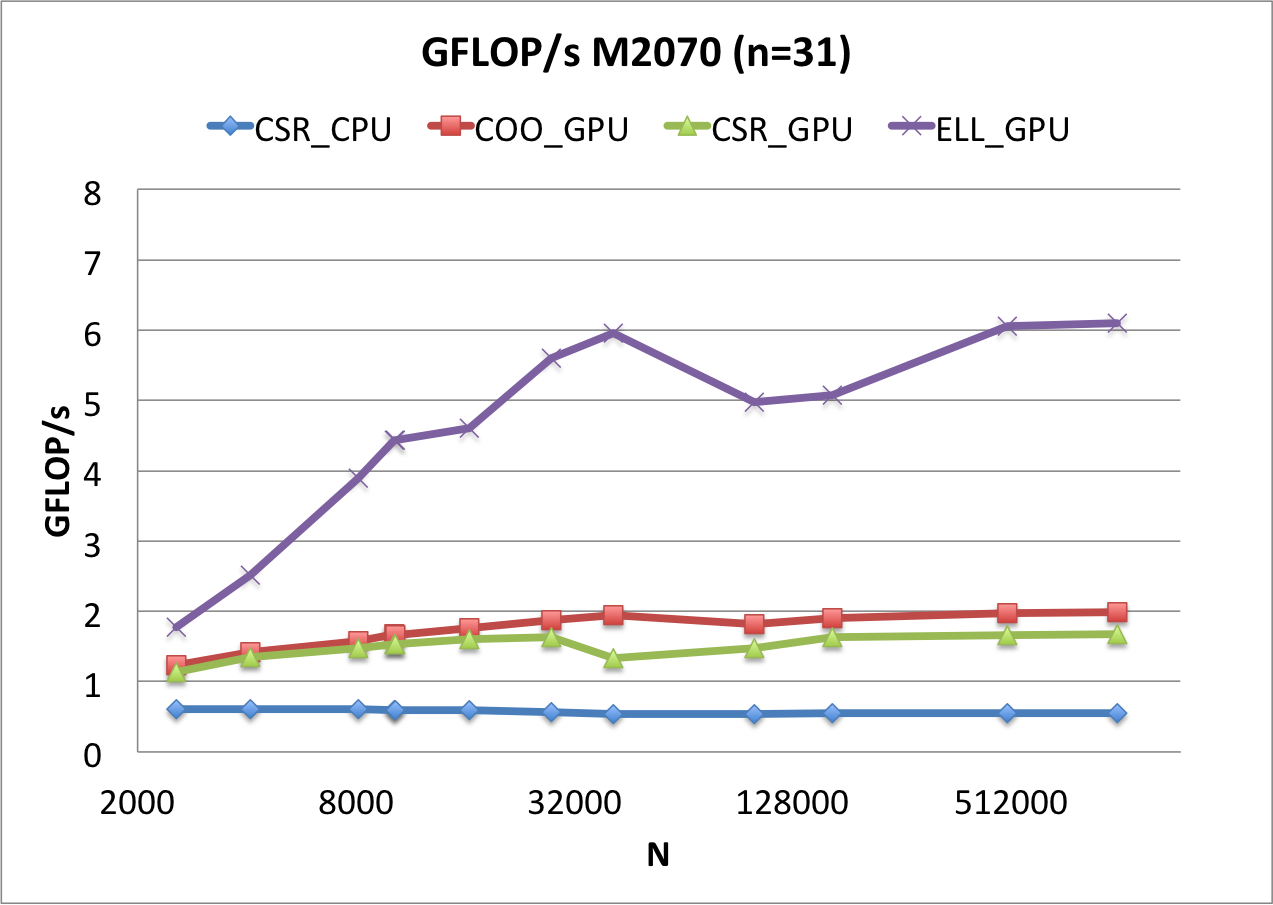
\includegraphics[width=\textwidth]{gpu_content/cascade_spmv/gflops_cascade_m2070_n31.png}
\caption{Stencil size $n=31$}
%\label{fig:gflops_cascade_m2070_n31}
\end{subfigure}
\begin{subfigure}[t]{0.48\textwidth}
\centering
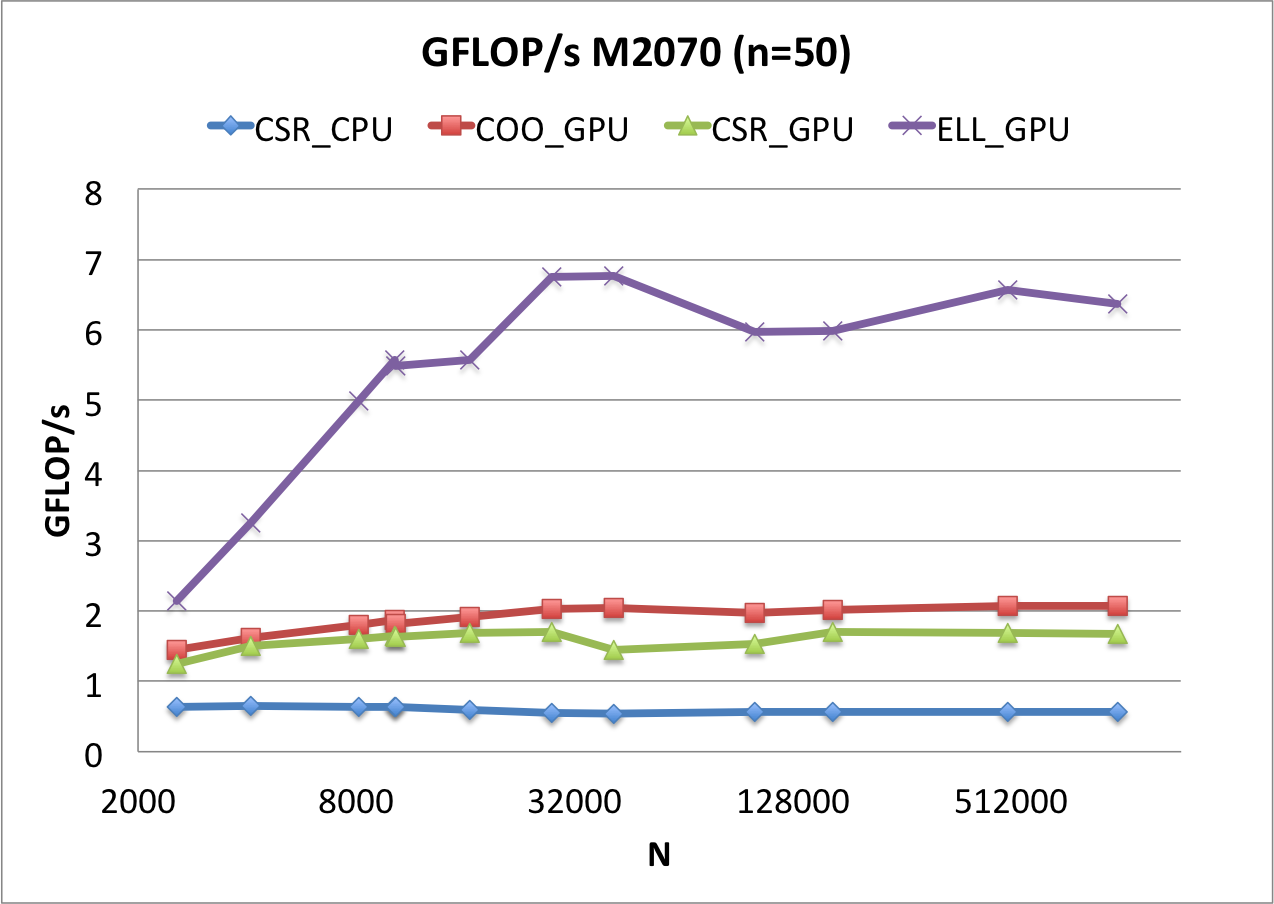
\includegraphics[width=\textwidth]{gpu_content/cascade_spmv/gflops_cascade_m2070_n50.png}
\caption{Stencil size $n=50$}
%\label{fig:gflops_cascade_m2070_n50}
\end{subfigure}
\quad
\begin{subfigure}[t]{0.48\textwidth}
\centering
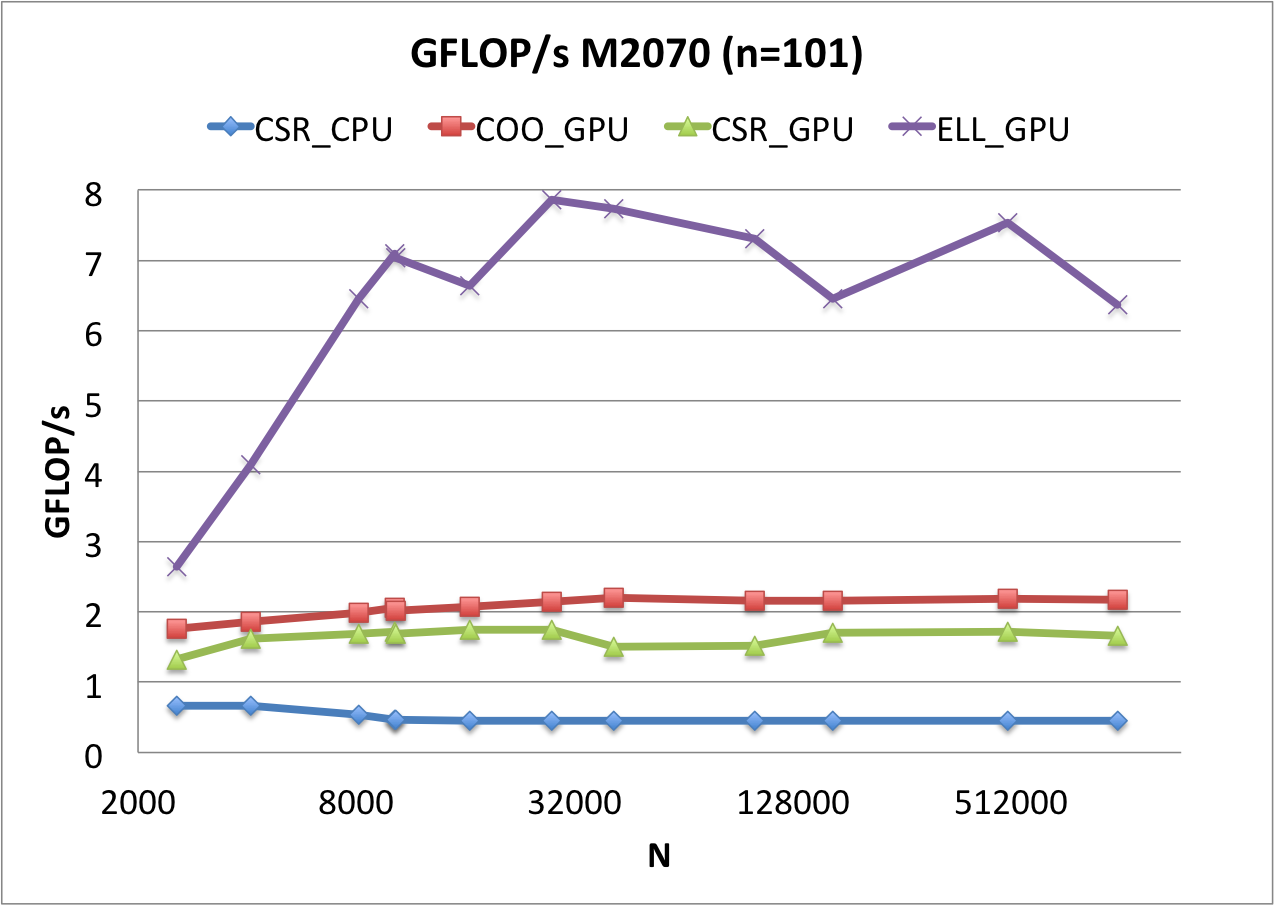
\includegraphics[width=\textwidth]{gpu_content/cascade_spmv/gflops_cascade_m2070_n101.png}
\caption{Stencil size $n=101$}
%\label{fig:gflops_cascade_m2070_n101}
\end{subfigure}
\caption{Performance comparison of CSR, COO and ELL matrix formats on Cascade's NVidia M2070 GPU and Intel Westmere CPU (Intel Xeon X5675).}
\label{fig:gflops_cascade_m2070}
\end{figure}


\begin{figure} 
\centering
\begin{subfigure}[t]{0.48\textwidth}
\centering
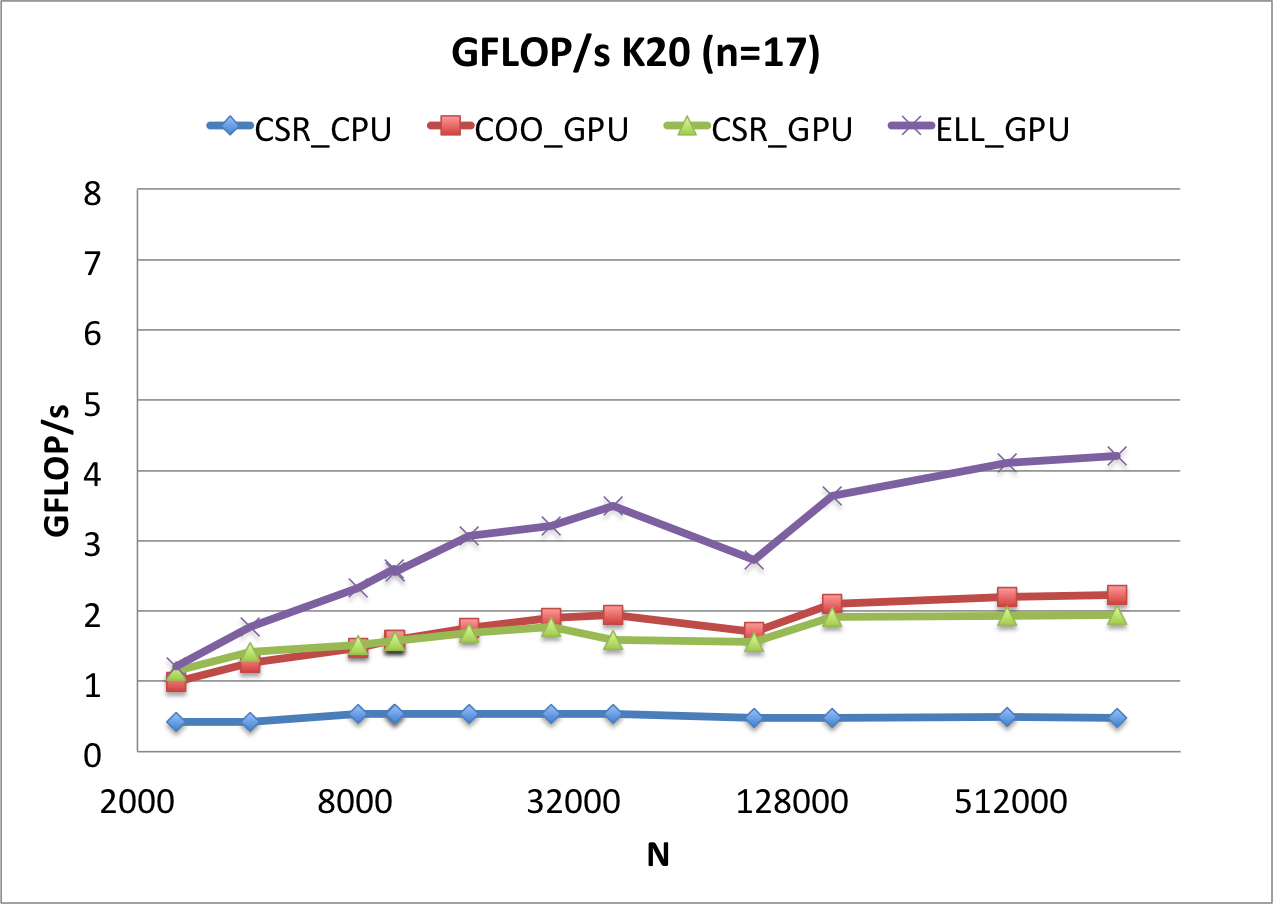
\includegraphics[width=\textwidth]{gpu_content/cascade_spmv/gflops_cascade_k20_n17.png}
\caption{Stencil size $n=17$}
%\label{fig:gflops_cascade_k20_n17}
\end{subfigure}
\quad
\begin{subfigure}[t]{0.48\textwidth}
\centering
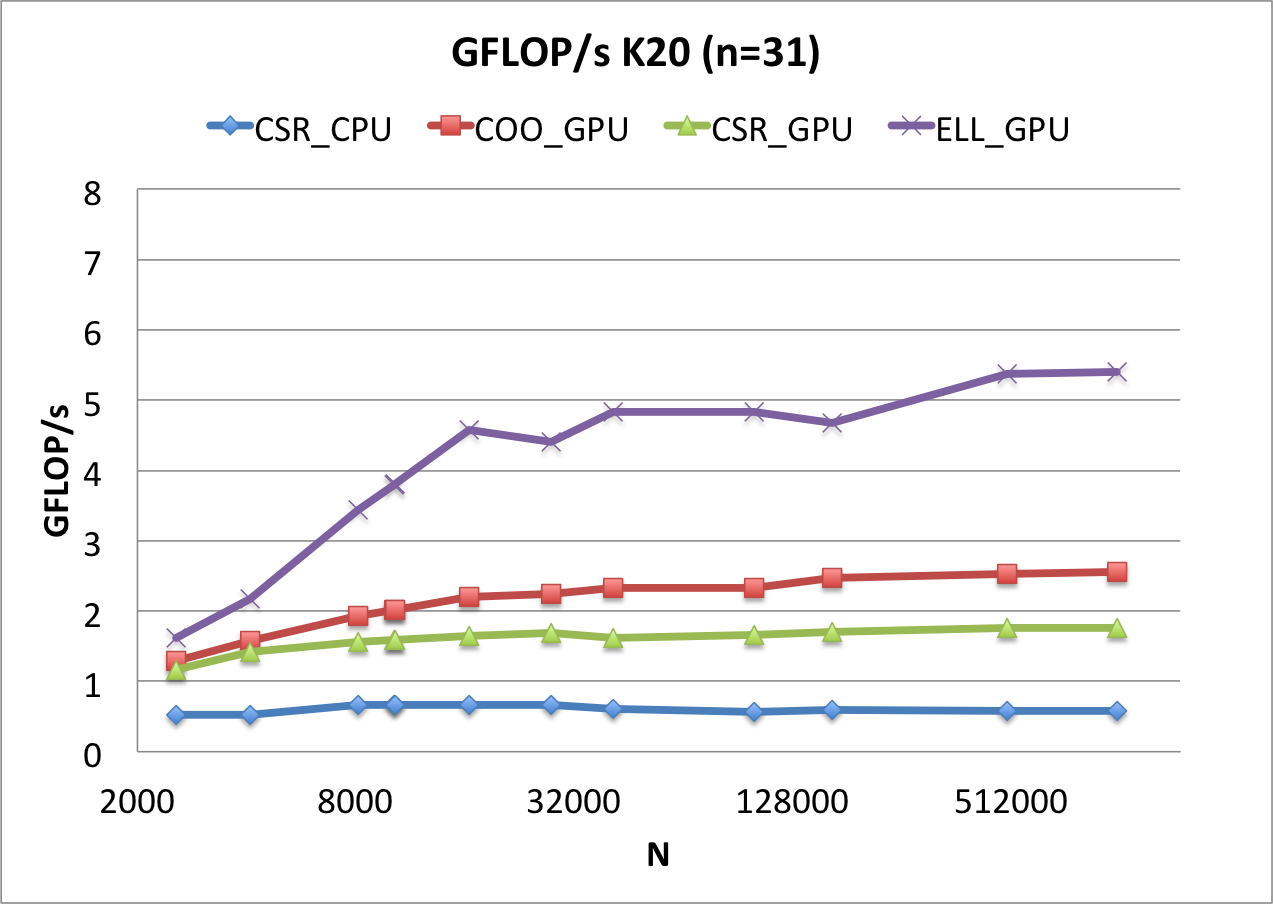
\includegraphics[width=\textwidth]{gpu_content/cascade_spmv/gflops_cascade_k20_n31.png}
\caption{Stencil size $n=31$}
%\label{fig:gflops_cascade_k20_n31}
\end{subfigure}
\begin{subfigure}[t]{0.48\textwidth}
\centering
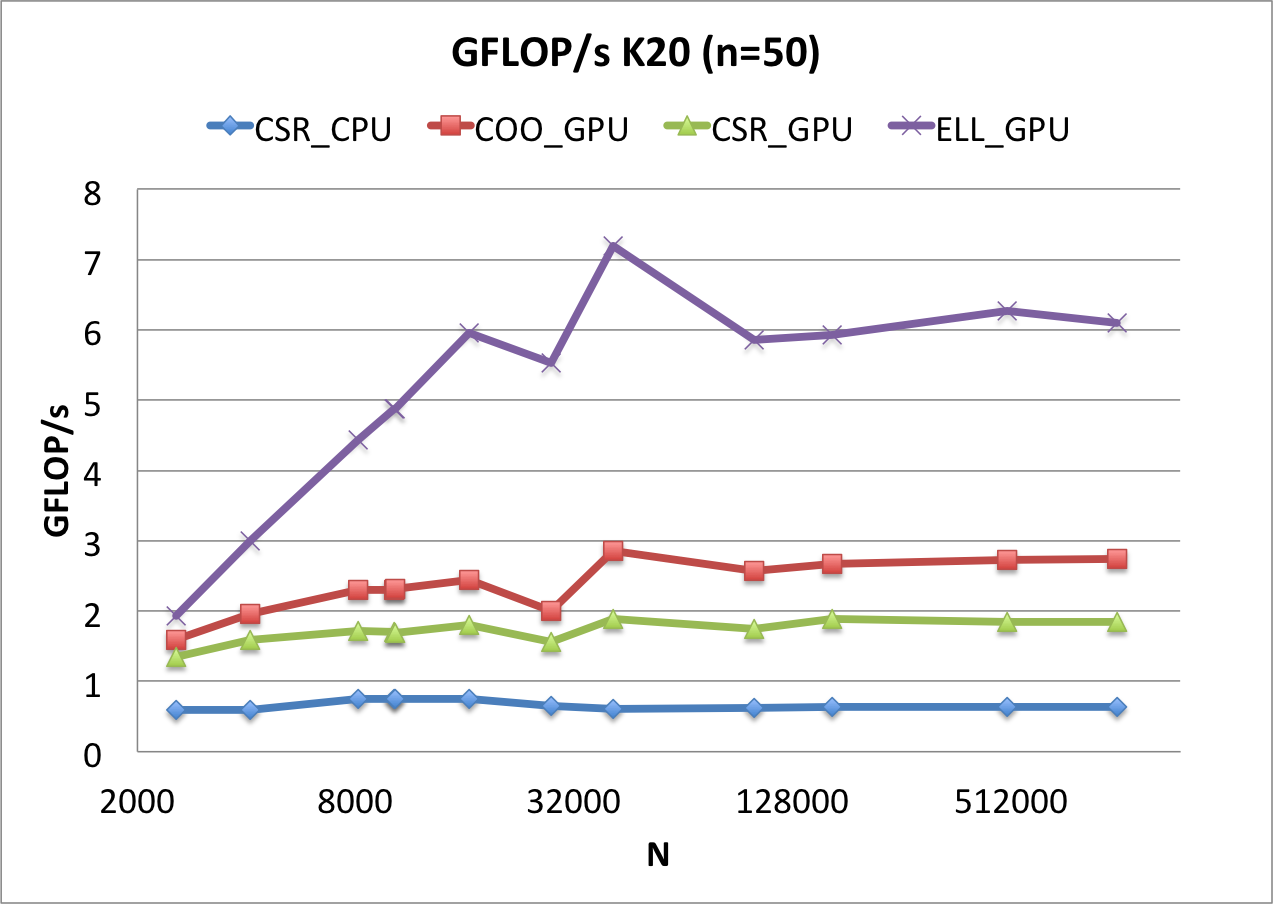
\includegraphics[width=\textwidth]{gpu_content/cascade_spmv/gflops_cascade_k20_n50.png}
\caption{Stencil size $n=50$}
%\label{fig:gflops_cascade_k20_n50}
\end{subfigure}
\quad
\begin{subfigure}[t]{0.48\textwidth}
\centering
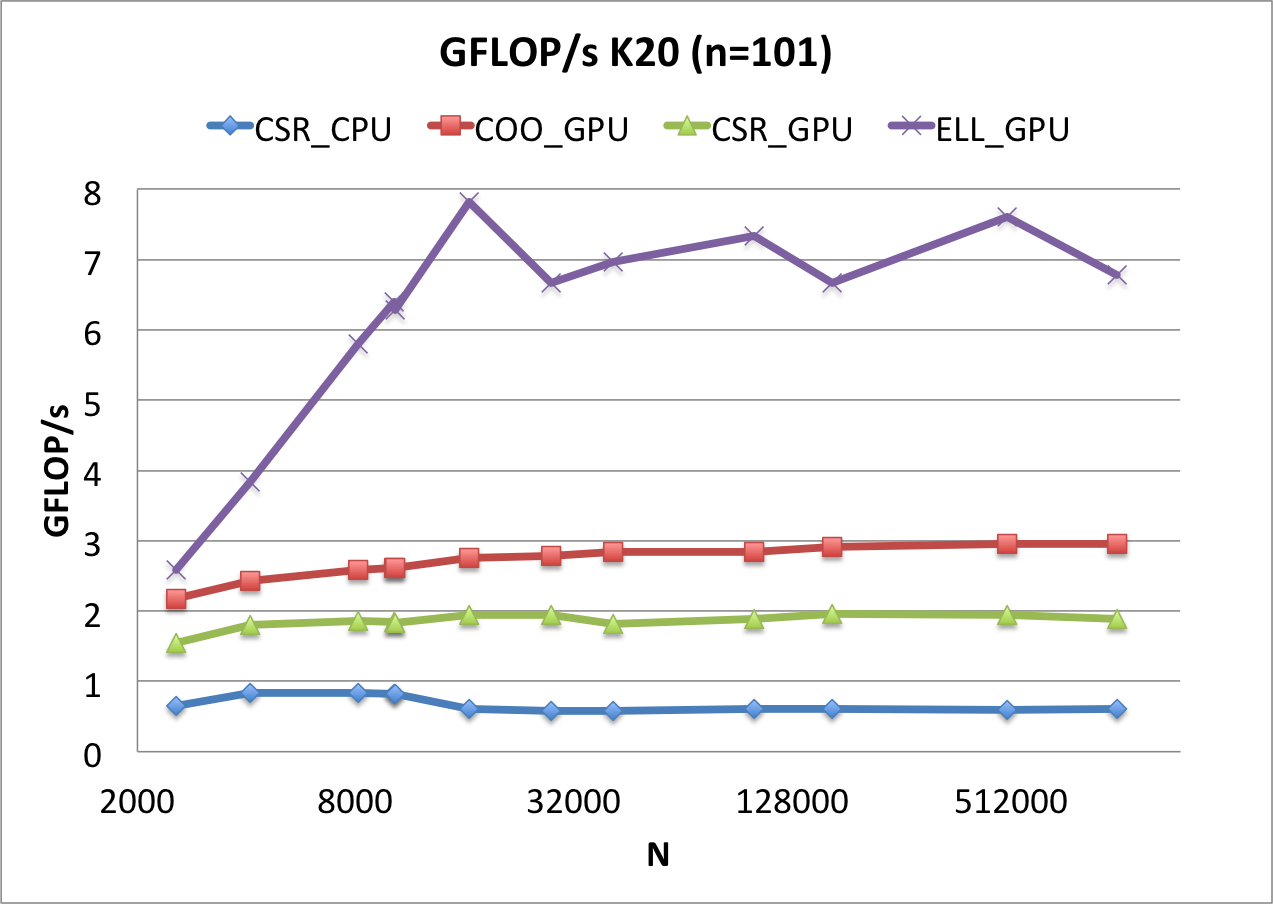
\includegraphics[width=\textwidth]{gpu_content/cascade_spmv/gflops_cascade_k20_n101.png}
\caption{Stencil size $n=101$}
%\label{fig:gflops_cascade_k20_n101}
\end{subfigure}
\caption{Performance comparison of ViennaCL CSR, COO and ELL matrix formats on Cascade's NVidia K20 GPU versus the Boost::uBLAS CSR format on and Intel Sandy-Bridge CPU (Intel Xeon E5-2670).}
\label{fig:gflops_cascade_k20}
\end{figure}


Figures~\ref{fig:ell_gflops_cascade_m2070} and \ref{fig:ell_gflops_cascade_k20} summarize the best achieved GFLOP/sec (in all cases the ELL format) for each stencil size on the M2070's and K20's respectively. Figures~\ref{fig:ell_speedup_cascade_m2070} and \ref{fig:ell_speedup_cascade_k20} show the achieved speedup each GPU gained over their respective Westmere and Sandy-Bridge CPUs. In the case of the K20, Figure~\ref{fig:ell_speedup_cascade_k20} shows that the Sandy-Bridge architecture is closing the divide between CPUs and GPUs, although an order of magnitude difference in the GFLOP/sec still exists.

\begin{figure} 
\centering
\begin{subfigure}[t]{0.48\textwidth}
\centering
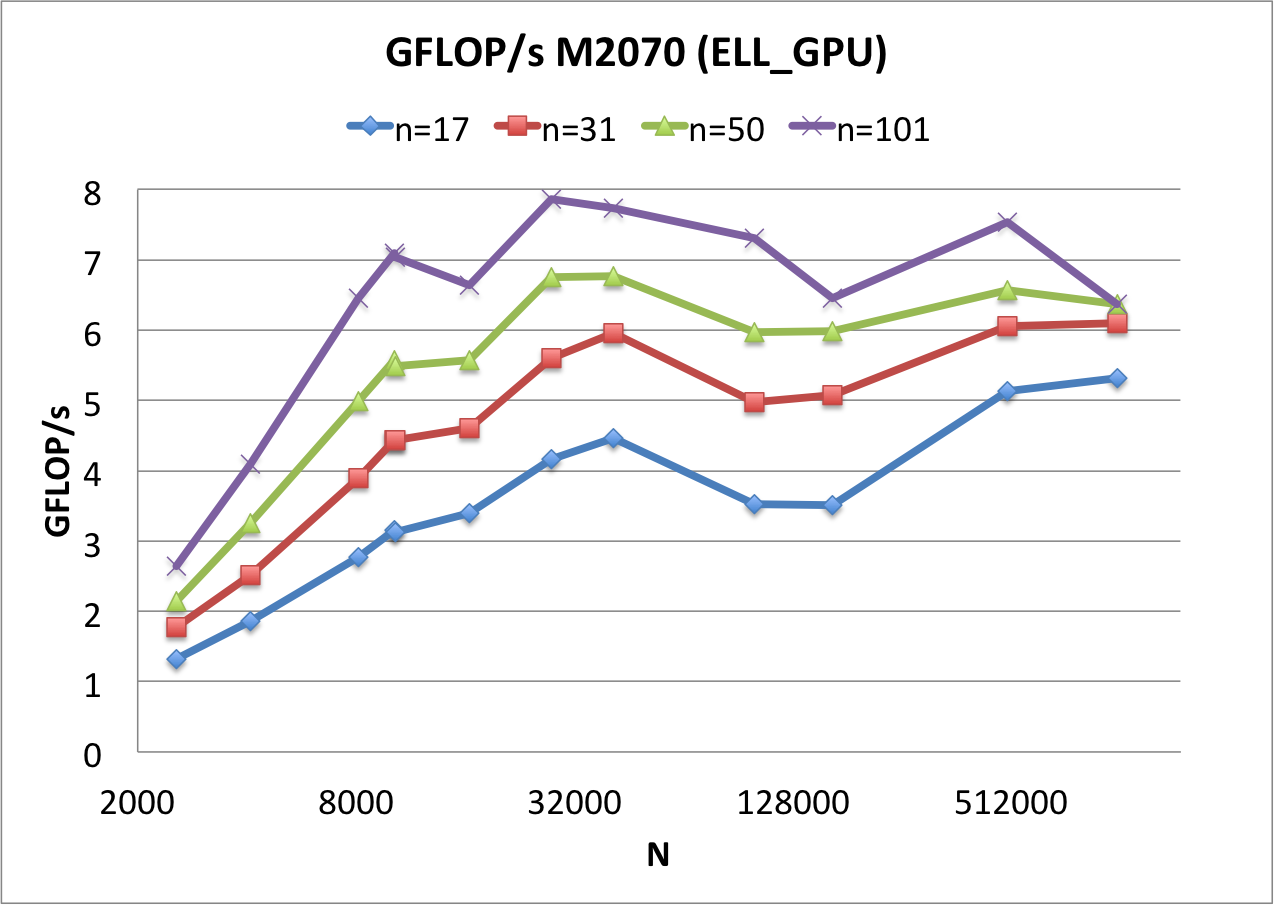
\includegraphics[width=\textwidth]{gpu_content/cascade_spmv/ell_comparison_cascade_m2070.png}
\caption{GFLOP/sec, NVidia M2070 GPU (Cascade)}
\label{fig:ell_gflops_cascade_m2070}
\end{subfigure}
\quad
\begin{subfigure}[t]{0.48\textwidth}
\centering
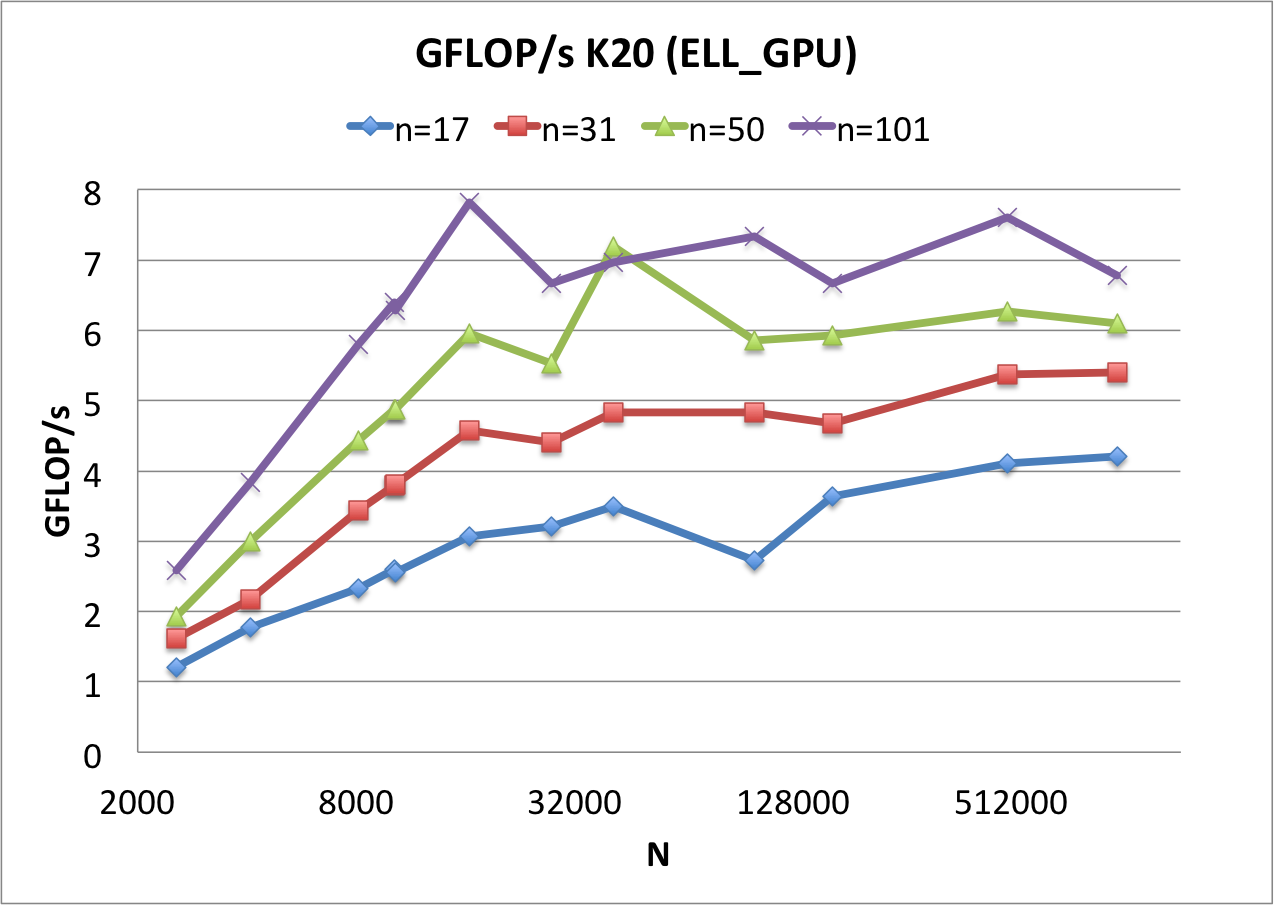
\includegraphics[width=\textwidth]{gpu_content/cascade_spmv/ell_comparison_cascade_k20.png}
\caption{GFLOP/sec, NVidia K20 GPU (Cascade)}
\label{fig:ell_gflops_cascade_k20}
\end{subfigure}
\begin{subfigure}[t]{0.48\textwidth}
\centering
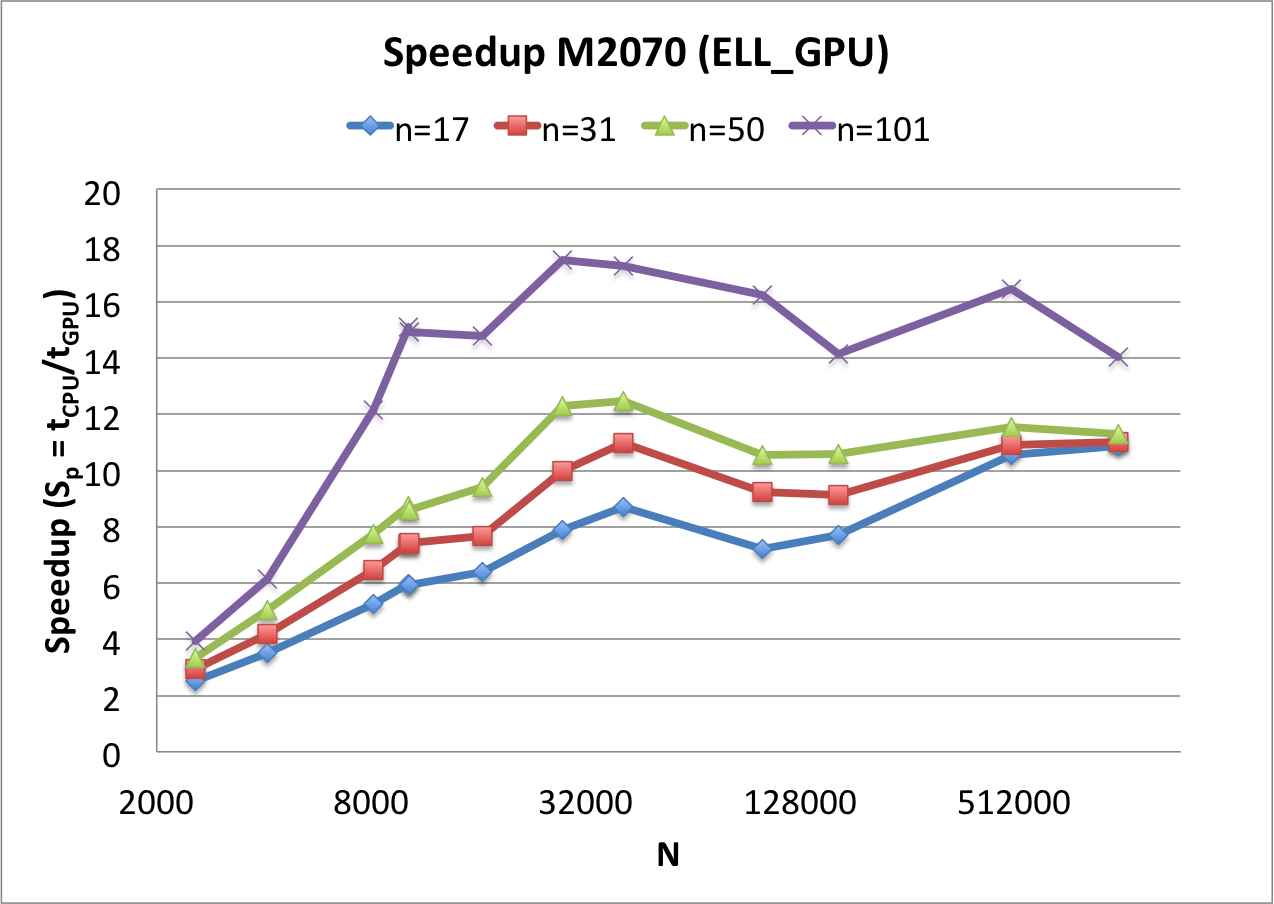
\includegraphics[width=\textwidth]{gpu_content/cascade_spmv/ell_comparison_speedup_cascade_m2070.png}
\caption{Speedup, NVidia M2070 GPU (Cascade) vs. CSR format on Intel Westmere (Intel Xeon X5675)}
\label{fig:ell_speedup_cascade_m2070}
\end{subfigure}
\quad
\begin{subfigure}[t]{0.48\textwidth}
\centering
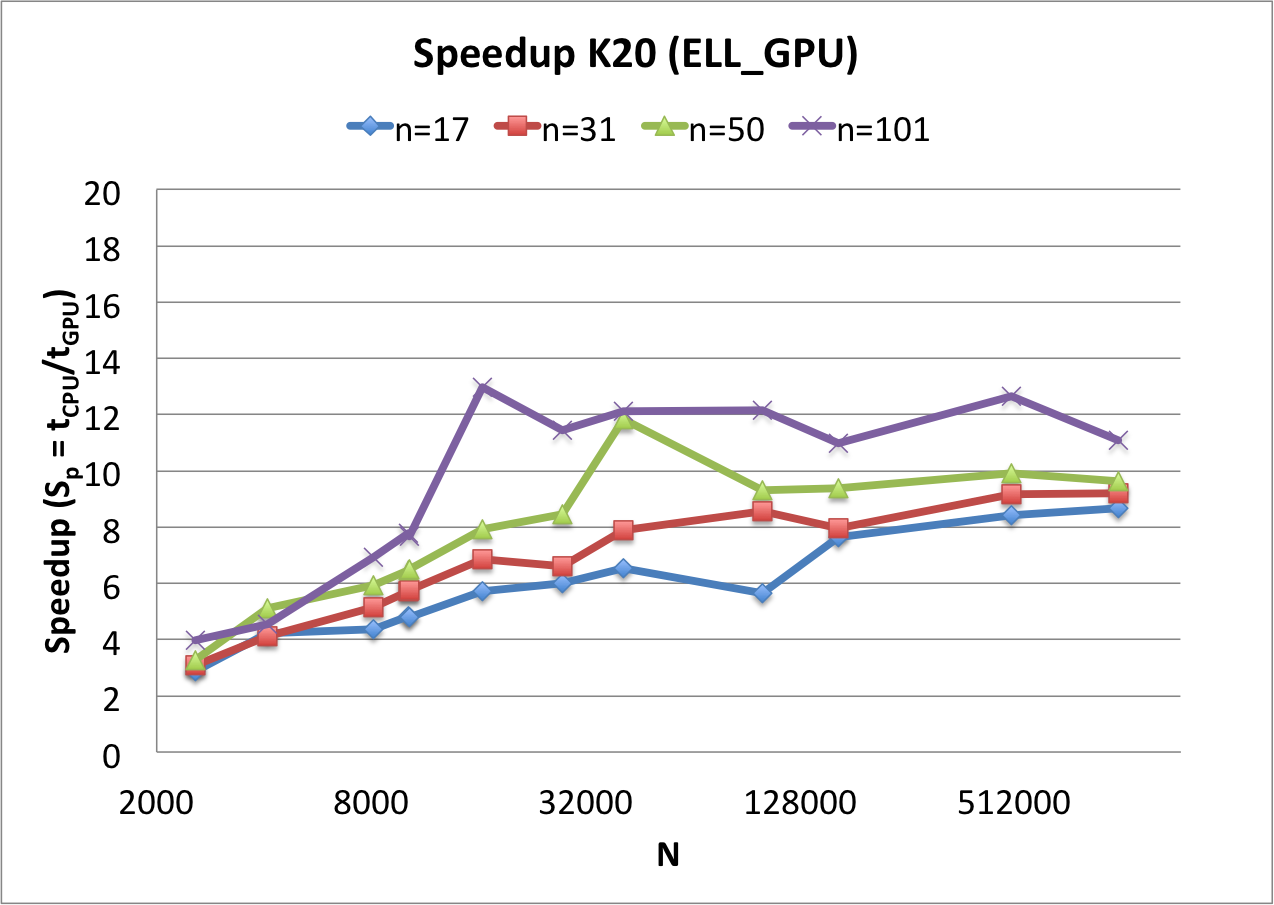
\includegraphics[width=\textwidth]{gpu_content/cascade_spmv/ell_comparison_speedup_cascade_k20.png}
\caption{Speedup, NVidia K20 GPU (Cascade) vs. CSR format on Sandy-Bridge (E5-2670)}
\label{fig:ell_speedup_cascade_k20}
\end{subfigure}
\caption{Comparison by stencil size for the ELL sparse matrix format.}
\end{figure}





\subsection{Intel Phi} 

As part of future work into accelerating RBF methods, investigations are underway into the new Intel Phi architecture. The variety of hardware available on Cascade will help us establish a clear argument in the choice of accelerator type and resolve the dilemma between choosing Phi vs GPU for our method. Since RBFs generalize other methods, our results should have broad reaching impact to answer similar questions for related methods.

%TODO: preliminary benchmarks on performance of ViennaCL SpMV. 

With the generalization of RBF-FD derivative computation formulated as a sparse matrix multiplication, we can 
% TODO: mention CUSP as alternative but concentrate on VCL
consider the various sparse formats provided by CUSP and ViennaCL. 

%TODO later: \item All stencils with non-uniform size
%TODO: What is the optimal choice of sparse container? How do the sparse containers compare in performance to each other, and to our custom kernels? What can we conclude? 


Figure~\ref{fig:gflops_cascade_intel_phi} is provided for comparison with Figures~\ref{fig:gflops_cascade_m2070} and \ref{fig:gflops_cascade_k20}. This stresses the point that although OpenCL offers functional portability, performance portability is still limited. 

\begin{figure} 
\centering
\begin{subfigure}[t]{0.48\textwidth}
\centering
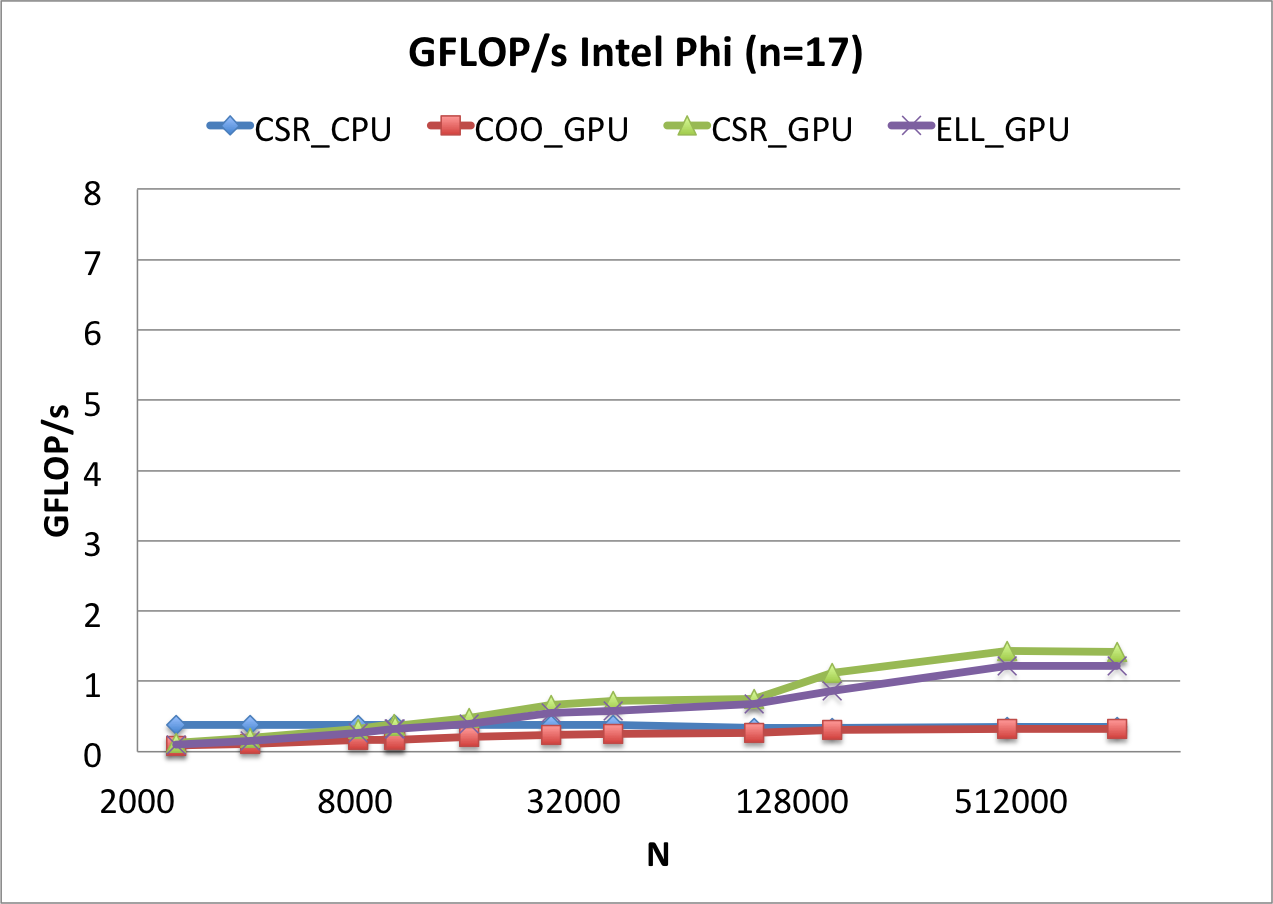
\includegraphics[width=\textwidth]{gpu_content/cascade_spmv/gflops_cascade_intel_phi_n17.png}
\caption{Stencil size $n=17$}
%\label{fig:gflops_cascade_intel_phi_n17}
\end{subfigure}
\quad
\begin{subfigure}[t]{0.48\textwidth}
\centering
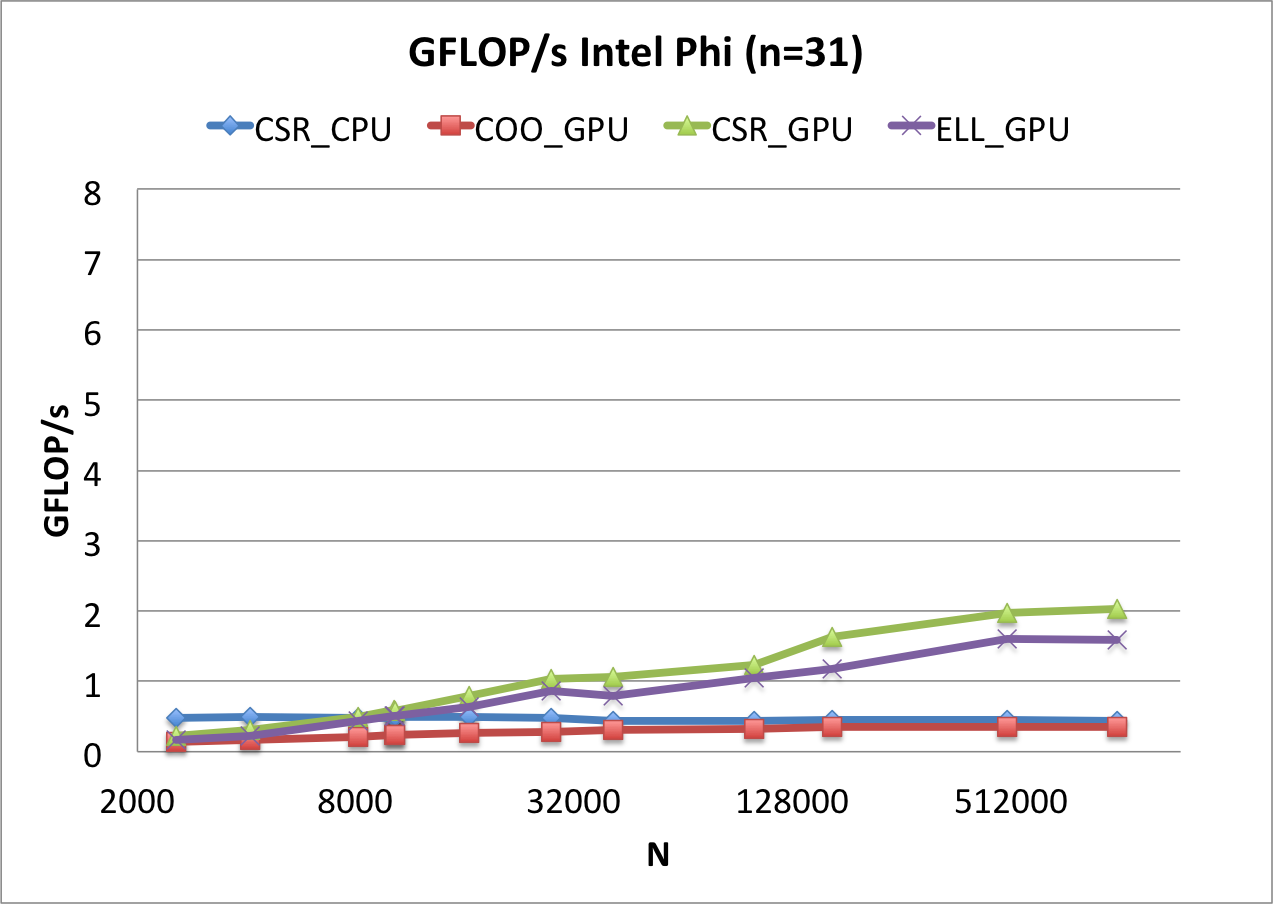
\includegraphics[width=\textwidth]{gpu_content/cascade_spmv/gflops_cascade_intel_phi_n31.png}
\caption{Stencil size $n=31$}
%\label{fig:gflops_cascade_intel_phi_n31}
\end{subfigure}
\begin{subfigure}[t]{0.48\textwidth}
\centering
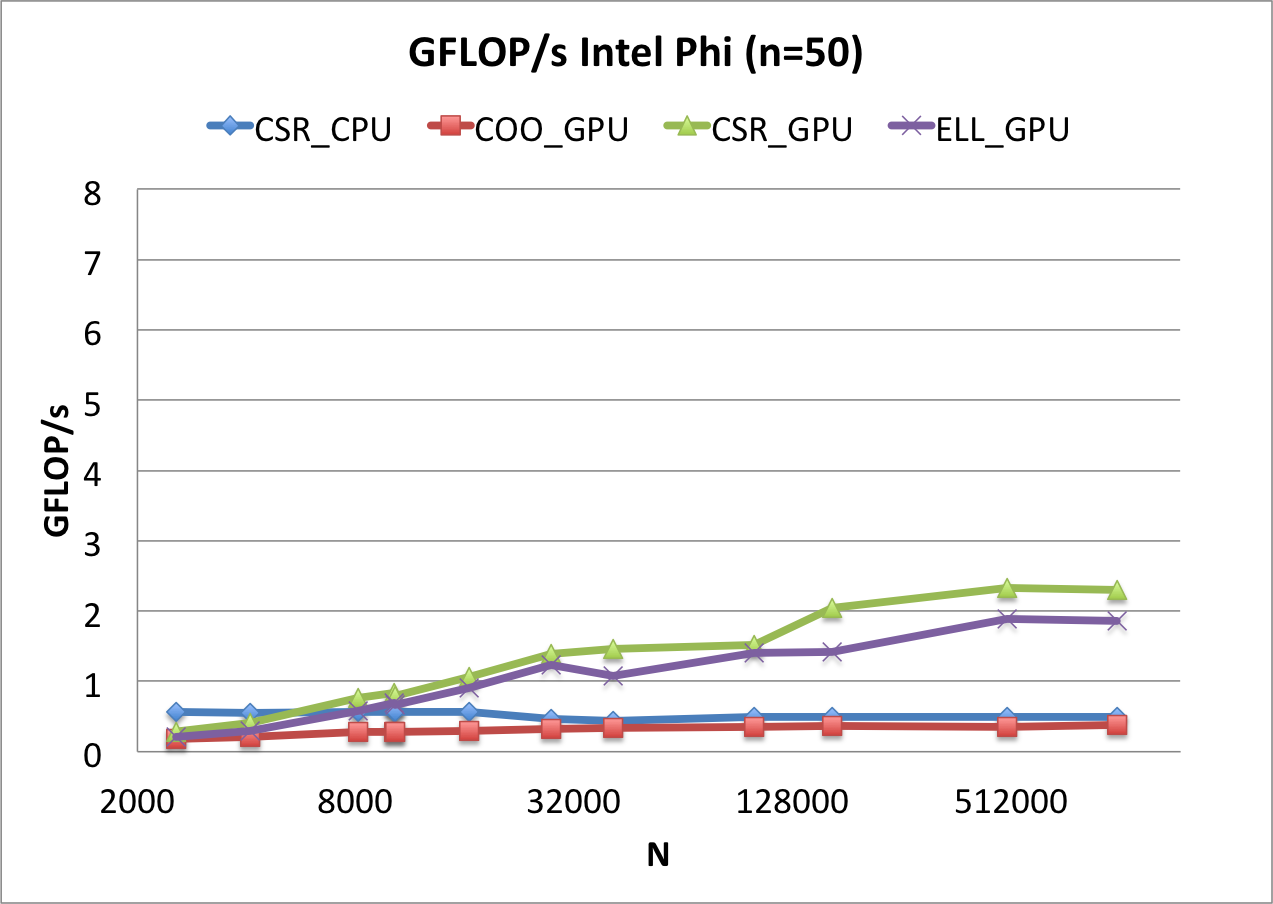
\includegraphics[width=\textwidth]{gpu_content/cascade_spmv/gflops_cascade_intel_phi_n50.png}
\caption{Stencil size $n=50$}
%\label{fig:gflops_cascade_intel_phi_n50}
\end{subfigure}
\quad
\begin{subfigure}[t]{0.48\textwidth}
\centering
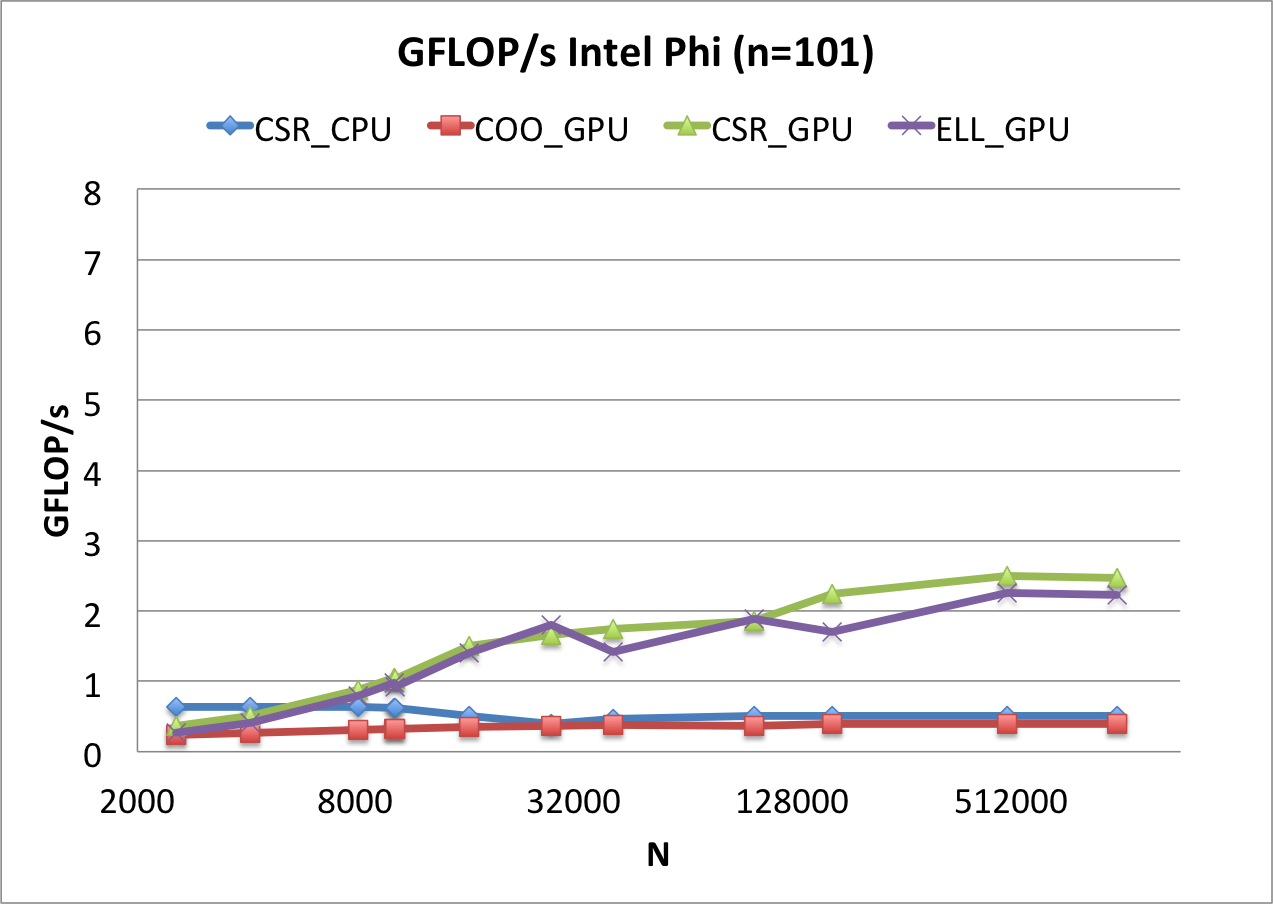
\includegraphics[width=\textwidth]{gpu_content/cascade_spmv/gflops_cascade_intel_phi_n101.png}
\caption{Stencil size $n=101$}
%\label{fig:gflops_cascade_intel_phi_n101}
\end{subfigure}
\caption{Performance comparison of ViennaCL CSR, COO and ELL matrix formats on Cascade's Intel Phi Accelerator, and the Boost::uBLAS CSR format on an Intel Sandy-Bridge CPU (Intel Xeon E5-2670). ViennaCL's kernels are optimized for NVidia GPUs, but function (albeit poorly) on the Intel Phi with the current release of Intel's OpenCL SDK (May, 2013). }
\label{fig:gflops_cascade_intel_phi}
\end{figure}




\section{Conclusions and Future Work}

This chapter presents the first implementation of RBF-FD to run on GPUs. Our OpenCL implementations apply RBF-FD differentiation matrices via Sparse Matrix-Vector multiplication (SpMV) to compute derivatives everywhere in the domain. The solution values are then updated via a fourth-order Runge Kutta (RK4) time-step. 

Two custom GPU SpMV kernels were tested: one that performs the SpMV by dedicating one thread to compute each row of the differentiation matrix, and one that applies 32 threads (a warp) to compute each row. 

The Roofline model (\cite{Williams2009}) was introduced to manage expectations for the peak possible performance (in terms of GFLOP/sec) that can be achieved for RBF-FD. Although GPUs advertise over 1 TFLOP/sec peak possible performance in double precision, the actual achieved FLOP/sec for the memory-bound RBF-FD application is significantly lower. The SpMV operational intensity of $\frac{1}{8}$ FLOPs:bytes, limits the expected performance to be less than 20 GFLOP/sec on NVidia M2070 hardware. Our custom OpenCL kernels achieve at most 3 GFLOP/sec on NVidia M2070 GPUs.



Sparse containers allow increased efficiency compared to our custom kernels. 
In an effort to boost performance, we integrated the ViennaCL library into our RBF-FD implementation and compared performance of three sparse containers provided by the library to determine the most appropriate sparse representation for RBF-FD. We compare the performance of the ViennaCL sparse containers (ELL, CSR, COO), and a CPU-only implementation of SpMV to the BOOST::uBLAS compressed-row storage. 

%ViennaCL allows control of the number of work-items for each kernel. 
%ViennaCL includes a set of auto-tuning options. %TODO: provide tuned parameters

%TODO: what is profile for each GPU type
%TODO: What is the significance of tuning on our problem $n=17, 31, 50, 101,$ etc. 
%TODO: experiment: SpMV on N=10^6, n = variable (5->105)
%TODO: idealized experiment: SpMV on N=10^6 regular grid with n=variable.








The latest version of OpenMP (v4.0) introduces pragmas for offloading computation to accelerators. These pragmas will function similarly to pragmas from PGI, OpenACC, and the Intel MIC. 


%
%
%Hardware architecture
%•	Memory layout
%•	Processing cores
%•	Trends in hardware since 2006 (additions and benfits)
%Optimization
%•	SpMV memory layout
%•	Scheduling threads
%•	Reductions
%OpenCL
%•	Why? 
%o	Cross platform support
%o	Asynchronous Queuing with Dependencies
%•	Implementations details
%o	Kernel
%o	Work-Item
%o	Work-Group
%o	NDRange
%o	Queue
%o	Etc.
%•	How does it compare to CUDA? Phi
%•	Latest trends
%o	Phi: bind against MKL for optimized CPU and MIC
%o	CUDA-MPI
%o	CUDA Sub-Kernel calls
%o	CUDA uptake 
%•	E.g., Matlab (MEX compiled kernel wrappers)
%Conclusions on GPGPU
%•	Benefits are good
%o	Cheap to purchase < $1K
%o	superior performance 1.2 TFLOPs possible in one card
%o	was a trending technology (major uptake in supercomputing and national labs)
%•	Downsides were varied
%•	Overall Impression is that
%o	Uptake was wide-spread for research projects
%o	Focus was on determining limits of the hardware
%•	Many studies focused on optimization of primitives which allow general use in applications such as RBF-FD without recreating the wheel when it comes to optimal algorithms. Allows researchers to concentrate on other investigations into application, preconditioning, data analysis, etc.
%Newcomers to the field are interested USING gpgpu applications, rather than writing them  


%TODO: put somewhere else
% When matrix is sparse, a direct LU decomposition causes fill-in on factorization. In some cases the fill-in can be minimal, but in general one must assume that fill in can turn the sparse matrix into a dense matrix. To invert and solve Equation~\ref{eq:implicit_eq}, use an iterative solver like GMRES. The GMRES algorithm (described further in Chapter~\ref{chap:applications} applies successive SpMVs along with other vector operations to converge on a solution. Due to the dominance of SpMV in GMRES, the performance of RBF-FD reduces once again to SpMV.



\ifstandalone
\bibliographystyle{plain}
\bibliography{merged_references}
\end{document}
\else
\expandafter\endinput
\fi


